% !TEX TS-program = xelatex
% !TEX encoding = UTF-8 Unicode

\documentclass[lang=cn,10pt]{elegantbook}

% 定义所有的图片文件在 figures 子目录下
\graphicspath{{figures/}}

\title{计算机图形学原理(虎书)}
\subtitle{Fundamentals of Computer Graphics}

\author{Steve Marschener \& Peter Shirley}
\institute{515}
\date{\the\year~年~\the\month~月~\the\day~日}
\version{0.0}
\bioinfo{译者}{Nancy Dong , Max Zhang}

\extrainfo{世界上只有一种英雄主义,那就是看清生活的真相之后依旧热爱生活。—— 罗曼罗兰}

\setcounter{tocdepth}{3}

\logo{logo-blue.png}
\cover{Tiger.png}

% 本文档命令
\usepackage{array}
\newcommand{\ccr}[1]{\makecell{{\color{#1}\rule{1cm}{1cm}}}}

% 修改标题页的橙色带
% \definecolor{customcolor}{RGB}{32,178,170}
% \colorlet{coverlinecolor}{customcolor}

\begin{document}
	
\maketitle
\frontmatter
	
\tableofcontents



\chapter*{前言}
\addcontentsline{toc}{chapter}{前言}

这一版的《计算机图形学基础》包含了对于材料着色、光反射、路径追踪的大量重写,以及从头至尾的更正。这一版书通过名为基于物理的材料和基于物理的渲染更好的介绍了计算机图形学技术,并且二者逐渐在实践中占据主导地位。现在这本材料被更好的整合了,我们认为这本书很好地反映了目前许多教师教授图形课程的组织大纲。

本书的结构与第四版基本相似。多年来我们对本书不断进行修订,我们努力保留了早期版本所特有的非正式、直观的表达方式,同时提高了一致性、精确性和完整性。我们希望在众多计算机图形学教材中,读者会觉得这本书是一个很有吸引力的平台。

\section*{关于封面}
\addcontentsline{toc}{section}{关于封面}

封面图片来自于J.W.Baker的《水中之虎》( \url{www.jwbart.com})

老虎的主题参考了Alain Fournier (1943-2000)于1998年在康奈尔大学的一次研讨会上发表的精彩演讲。他的演讲是关于老虎运动的,是一个令人回味无穷的描述。他总结了自己的观点:

尽管在过去的35年中,计算机图形学的建模和渲染已经得到了极大的改进,但我们仍然无法自动模拟出在河中游泳老虎的所有精彩细节。自动是指不需要艺术家/专家仔细的进行手动调整。

坏消息是我们还有很长的路要走。

好消息是我们还有很长的路要走。

\section*{在线资源}

本书的网址是\url{http://www.cs.cornell.edu/~srm/fcg5/}。我们将继续维护勘误表和那些使用本书的课程链接,以及与本书风格相匹配的教材。本书中的大多数图片都是Adobe Illustrator格式,我们很乐意根据要求将指定的图片转换为可移植格式。请随时通过shirley@cs.utah.edu 或 srm@cs.cornell.edu 与我们联系。

\section*{致谢}

以下人员提供了有关本书各个版本的有用信息、评论或反馈:Ahmet O\u{g}uz Aky{\"u}z, Josh Andersen, Beatriz Trinch\~ao Andrade Zeferino Andrade, Bagossy Attila, Kavita Bala, Mick Beaver, Robert Belleman, Adam Berger, Adeel Bhutta, Solomon Boulos, Stephen Chenney, Michael Coblenz, Greg Coombe, Frederic Cremer, Brian Curtin, Dave Edwards, Jonathon Evans, Karen Feinauer, Claude Fuhrer, Yotam Gingold, Amy Gooch, Eungyoung Han, Chuck Hansen, Andy Hanson, Razen Al Harbi, Dave Hart, John Hart, Yong Huang, John “Spike” Hughes, Helen Hu, Vicki Interrante, Wenzel Jakob, Doug James, Henrik Wann Jensen, Shi Jin, Mark Johnson, Ray Jones, Revant Kapoor, Kristin Kerr, Erum Arif Khan, Mark Kilgard, Fangjun Kuang, Dylan Lacewell, Mathias Lang, Philippe Laval, Joshua Levine, Marc Levoy, Howard Lo, Joann Luu, Mauricio Maurer, Andrew Medlin, Ron Metoyer, Keith Morley, Eric Mortensen, Koji Nakamaru, Micah Neilson, Blake Nelson,
Michael Nikelsky, James O'Brien, Hongshu Pan , Steve Parker, Sumanta Pattanaik, Matt Pharr, Ken Phillis Jr,  Nicol{\`o} Pinciroli, Peter Poulos, Shaun Ramsey, Rich Riesenfeld, Nate Robins, Nan Schaller, Chris Schryvers, Tom Sederberg, Richard Sharp, Sarah Shirley, Peter Pike Sloan, Hannah Story, Tony Tahbaz, Jan Phillip Tiesel, Bruce Walter, Alex Williams, Amy Williams, Chris Wyman, Kate Zebrose, Angela Zhang。

Ching-Kuang Shene和David Solomon允许我们借用他们的例子。Henrik Wann Jensen、Eric Levin、Matt Pharr和Jason Waltman慷慨地提供了图片。Brandon Mansfield帮助改进了关于光线追踪的分层包围体的讨论。Philip Greenspun (\url{philip.greenspun.com})好心地允许我们使用他的照片。John "Spike" Hughes帮助改进了对抽样理论的讨论。Wenzel Jakob的Mitsuba渲染器在帮助我们创作照片方面非常宝贵。我们非常感谢J.W. Baker帮助创作了Pete设想的封面。抛开他才华横溢艺术家的身份,与他个人合作也是一种极大的乐趣。

章节注释中引用了许多有助于编写本书的作品。然而,一些影响内容和表达的关键书籍值得特别关注。其中包括两个经典的计算机图形学书籍,我们从两本书中学习了基础知识:计算机图形术:\textit{Computer Graphics: Principles \& Practice(Foley、Van Dam、Feiner和Hughes,1990)}和\textit{ Computer Graphics (Hearn \& Baker, 1986)},Hill 的 \textit{Computer Graphics Using OpenGL (Francis S. Hill, 2000)},Angel 的 \textit{Interactive Computer Graphics: A Top-Down Approach Using OpenGL (Angel, 2002)}, Hugues Hoppe的华盛顿大学论文(Hoppe, 1994),Rogers的两篇优秀的图形学文章(D. F. Rogers, 1985, 1989)。

我们要特别感谢Alice和Klaus Peters,感谢他们鼓励Pete编写本书的第一版,并感谢他们在完成一本书方面的高超技巧。他们对作者的耐心,以及他们致力于让自己的书尽可能地做到最好的态度,对这本书的成功起到了至关重要的作用。没有他们非凡的努力,这本书无法完成。


\section*{译者续}

本书翻译著名的\textit{Fundamentals of Computer Graphics}(计算机图形学原理,虎书),水平有限,最大的目的是为了学习。

译者贡献列表(实时更新):

\begin{itemize}
	\item Nancy Dong
	\item Max Zhang
\end{itemize}

	
\mainmatter
	



\chapter{介绍}
\label{chap01}

“计算机图形学(Computer graphics)”一词描述了计算机创造和操纵图像的任何用途。本书介绍了算法和数学工具,可用于创建各种图像、逼真的视觉效果、信息丰富的技术插图或漂亮的计算机动画。图形可以是二维或三维的;图像可以是完全合成的,也可以通过对照片进行处理而生成。这本书是关于基础算法与数学的,特别是那些用来生成三维物体和景象的算法。

实际上,做计算机图形不可避免地需要了解特定的硬件、文件格式,通常还需要了解一两个图形API(参见第1.3节)。计算机图形学是一个快速发展的领域,所以对于该领域的学习是无止境的。因此,在这本书中,我们尽力避免依赖任何特定的硬件或API\footnote{API:应用程序接口(application program interface)}。我们也支持鼓励读者为其软件和硬件环境补充相关文档。幸运的是,计算机图形学有足够的标准术语和概念,本书的讨论应该很好地映射到大多数环境。

本章定义了计算机图形学的一些基本术语,并介绍了一些背景,以及与计算机图形学有关的资料来源。

\section{图形领域(Graphics Areas)}

在任何行业领域中硬性的分类都是不合理的,但大多数图形学研究者认同以下是计算机图形学核心领域:

\begin{itemize}
	\item \textbf{\textcolor{ForestGreen}{建模(Modeling)}}是以可存储在计算机上的方式处理形状和外观特性的数学规范。例如,一个咖啡杯可以被描述为一组有序的3D点,以及一些如何连接这些点的插值规则和一个描述光线如何与杯子相互作用的反射模型。
	
	\item \textbf{\textcolor{ForestGreen}{渲染(Rendering)}}是从艺术领域借鉴而来的术语,涉及到从三维计算机模型中创建着色图像。
	
	\item \textbf{\textcolor{ForestGreen}{动画(Animation)}}是一种通过图像序列创造运动幻象的技术。动画使用建模和渲染,但增加了如何随时间移动的关键问题,而这通常在基本建模和渲染中不会处理。
\end{itemize}

还有许多其他涉及计算机图形的领域,而它们是否属于核心图形领域,见仁见智。这些都将至少在正文中有所涉及。这些相关领域包括以下内容:

\begin{itemize}
	\item \textbf{\textcolor{ForestGreen}{用户交互(User interaction)}}涉及输入设备(如鼠标和平板电脑)、应用程序、图像中对用户的反馈以及其他感官反馈之间的界面。从历史上看,这一领域与图形学有关,主要是因为图形学研究人员最早接触到了现在无处不在的输入/输出设备。

	\item \textbf{\textcolor{ForestGreen}{虚拟现实(Virtual reality)}}试图让用户沉浸在一个三维虚拟世界中。这通常要求至少有立体图形和对头部运动的反应。对于真正的虚拟现实,还应该提供声音和力反馈。因为这一领域需要先进的3D图形和先进的显示技术,所以它通常与图形密切相关。

	\item \textbf{\textcolor{ForestGreen}{可视化(Visualization)}}试图通过视觉显示让用户深入了解复杂的信息。通常,在可视化问题中有很多图形问题需要解决。

	\item \textbf{\textcolor{ForestGreen}{图像处理(Image processing)}}涉及对二维图像的操作,在图形和视觉领域都有应用。

	\item \textbf{\textcolor{ForestGreen}{3D扫描(3D scanning)}}使用测距技术来创建测量的三维模型。这样的模型对于创造丰富的视觉图像很有帮助,而对这种模型的处理往往需要图形算法。

	\item \textbf{\textcolor{ForestGreen}{计算型摄影(Computational photography)}}是使用计算机图形、计算机视觉和图像处理方法,以实现拍摄物体、场景和环境的新方法。

\end{itemize}

\section{主要的应用领域(Major Applications)}

几乎任何工作都可以在一定程度上使用计算机图形,但计算机图形技术的主要用户包括以下行业:

\begin{itemize}
	\item \textbf{\textcolor{ForestGreen}{电子游戏(Video games)}}越来越多地使用复杂的3D建模和渲染算法。
	
	\item \textbf{\textcolor{ForestGreen}{动画片(Cartoons)}}通常是直接从3D模型中渲染出来的。许多传统的二维动画片使用由三维模型渲染的背景,这使得在不需要艺术家大量时间的情况下允许视点连续移动。
	
	\item \textbf{\textcolor{ForestGreen}{视觉特效(Visual effects)}}几乎使用所有类型的计算机图形学技术。几乎每部现代电影都使用数字合成技术,将背景与单独拍摄的前景叠加在一起。许多电影还使用三维建模和动画来创造合成环境、物体,甚至大多数观众永远不会怀疑的角色不是真实的。

	\item \textbf{\textcolor{ForestGreen}{动画电影(Animated films)}}使用了许多与视觉特效相同的技术,但不一定要以看起来图像更真实为目标。
	
	\item \textbf{\textcolor{ForestGreen}{计算机辅助设计和计算机辅助制造(CAD/CAM)}}这些领域使用计算机技术在计算机上设计零件和产品,然后使用这些虚拟设计来指导制造过程。例如,许多机械零件在3D计算机建模软件中设计,然后在计算机控制的铣削设备上自动生产。
	
	\item \textbf{\textcolor{ForestGreen}{仿真模拟(Simulation)}}可以被认为是精确的游戏。例如,飞行模拟器使用复杂的3D图形来模拟驾驶飞机的体验。这种模拟对于安全关键领域(如驾驶)的初始培训以及有经验用户的情景培训(如成本太高或太危险而无法实际创建的特定消防情况)非常有用。
	
	\item \textbf{\textcolor{ForestGreen}{医学成像(Medical imaging)}}通过扫描患者产生的数据创建有价值的图像。例如,计算机断层扫描(CT)数据集由大型3D密度值矩阵组成。计算机图形学被用来创建阴影图像,帮助医生从这些数据中提取最重要的信息。
	
	\item \textbf{\textcolor{ForestGreen}{信息可视化(Information visualization)}}创建的数据图像不一定具有“自然”的视觉描述。例如,十种不同股票价格的时间趋势没有明显的视觉描述,但巧妙的图形技术可以帮助人类看到这些数据中的模式。
\end{itemize}


\section{图形应用程序接口(Graphics APIs)}

使用图形库的一个关键部分是处理图形API。应用程序接口(API)是执行一组相关操作的标准函数集合,图形API是执行基本操作的一组函数,例如将图像和3D表面绘制到屏幕上的窗口中。

每个图形程序都需要能够使用两个相关的API:一个用于可视化输出的图形API和一个用于获取用户输入的用户界面API。目前,图形和用户界面API有两种主流模式。第一种是集成方法,以Java为例,其中图形和用户界面工具包是集成的、可移植的包,完全标准化并作为语言的一部分得到支持。第二种以Direct3D和OpenGL为代表,其中绘图命令是与C++等语言相关的软件库的一部分,用户界面软件是一个独立的实体,可能因系统而异。在后一种方法中,编写可移植代码是有问题的,尽管对于简单的程序,可以使用可移植库层来封装系统特定的用户界面代码。

无论选择哪种API,基本的图形调用基本上都是一样的,本书的概念也适用。

\section{图形管线(Graphics Pipeline)}

如今,每台台式电脑都有强大的3D图形管道。这是一个特殊的软件/硬件子系统,可以有效地绘制透视图中的三维图元。通常,这些系统针对处理具有共享顶点的3D三角形进行了优化。管线中基本操作是将三维的顶点位置映射到二维的屏幕位置,并对三角形进行着色,以使它们看起来真实,并以正确的前后顺序显示。

尽管以正确的前后顺序绘制三角形曾经是计算机图形学中最重要的研究问题,但现在大多是使用深度缓冲(z-buffer)来解决,其使用一种特殊的内存缓冲区,并且以暴力方式解决问题。

事实证明,在图形管线中使用的几何操作几乎完全可以在4D坐标空间中完成,该空间由3D坐标和有利于透视观察(perspective viewing)的第四个齐次坐标(homogeneous coordinate)组成。这些4D坐标使用4 × 4矩阵和4个向量来操作。因此,图形管线中包含许多用于高效处理这种矩阵和向量的计算单元。这个4D坐标系是计算机科学中使用的最微妙和最美丽的构造之一,它当然是学习计算机图形学时要跳过的最大的障碍。每本图形学书第一部分的很多内容都是关于4D坐标的。

生成图像的速度很大程度上取决于绘制三角形的数量。因为在许多应用程序中,交互性比视觉效果更重要,所以尽量减少用于表示模型的三角形数量是值得的。此外,如果从远处观察模型,比从近处观察模型需要更少的三角形。这表明用多细节层次(level of detail,LOD)来表示模型是有用的。

\section{数值问题(Numerical Issues)}

许多图形程序实际上只是3D数值代码。在这样的程序中,数值问题通常是至关重要的。在“过去”,以健壮和可移植的方式处理这样的问题是非常困难的,因为机器对数有不同的内部表示,更糟糕的是,处理异常的方式不同,且不兼容。幸运的是,几乎所有的现代计算机都符合IEEE浮点标准(IEEE Standards Association,1985)。这使得程序员可以对如何处理某些数字条件做出许多方便的假设。

虽然IEEE浮点有很多特性,在编码数字算法时很有价值,但在图形学中遇到的大多数情况下,只有少数几个特性是必须知道的。首先,也是最重要的一点,就是要了解IEEE浮点中的实数有三个“特殊”值:

\begin{enumerate}
	\item \textcolor{ForestGreen}{无穷大(Infinity,$\infty$)}这是一个有效的数字,比其他所有有效的数字都大。
	
	\item \textcolor{ForestGreen}{负无穷大(Minus infinity,$-\infty$)}这是一个有效的数字,比其他所有的有效数字都小。
	
	\item \textcolor{ForestGreen}{非数值形式(NaN)}这是一个无效的数字,产生于一个后果未定的操作,如零除以零。
\end{enumerate}


IEEE浮点的设计者做出了一些非常方便程序员的决定。其中许多与上述三个特殊值有关,用于处理除零等异常。在这些情况下,会记录一个异常,但在许多情况下,程序员可以忽略它。具体来说,对于任何正实数$a$,以下涉及除以无限值的规则成立\footnote{IEEE浮点有两种零的表示方法,一种是被视为正数,一种是被视为负数。虽然-0和+0之间的区别只是偶尔会出现,但在出现时还是值得记住的。}:


\begin{equation}
	\begin{aligned}	
		+a/(+\infty)=+0 \\
		-a/(+\infty)=-0 \\
		+a/(-\infty)=-0 \\
		-a/(-\infty)=+0 \\
	\end{aligned}
	\nonumber	
\end{equation}

其他涉及无限值的操作的行为也是可预测的。同样对于正数$a$,行为如下:

\begin{equation}
	\begin{aligned}	
		\infty+\infty&=+\infty\\
		\infty-\infty&= \rm NaN\\
		\infty*\infty&=\infty\\
		\infty/\infty&= \rm NaN \\
		\infty/a&=\rm NaN \\
		\infty/0&=\rm NaN \\
		0/0&=\rm NaN \\
	\end{aligned}
	\nonumber	
\end{equation}

布尔表达式中涉及无限值的规则如下所示:

\begin{enumerate}
	\item 所有有限的有效数字都小于正无穷。
	\item 所有有限的有效数字都大于负无穷。
	\item 负无穷比正无穷小。
\end{enumerate}

涉及有NaN值的表达式的规则很简单:

\begin{enumerate}
	\item 任何包含NaN的算术表达式的结果都是NaN。
	
	\item 任何涉及NaN的布尔表达式都是假的。
\end{enumerate}

IEEE浮点数最有用的方面也许是如何处理除以零的问题;对于任何正实数$a$,以下涉及除以零的规则是成立的:

\begin{equation}
	\begin{aligned}	
		+a/+0=+	\infty\\
		-a/+0=-	\infty
	\end{aligned}
\nonumber
\end{equation}

如果程序员利用IEEE规则,有许多数字计算会变得简单得多。例如,考虑表达式:

\begin{equation}\label{key}
	\begin{aligned}	
		a=\frac{1}{\frac{1}{b}+\frac{1}{c}}
	\end{aligned}
\nonumber
\end{equation}

电阻器和透镜会产生这样的表达式。如果除以零导致程序崩溃(在IEEE浮点之前的许多系统中都是如此),则需要两个If语句来检查$b$或$c$是否是小值或零值。相反,在IEEE浮点中,如果$b$或$c$为零,我们将根据需要获得$a$的零值。另一种避免特殊检查的常见技术是利用NaN的布尔属性。考虑以下代码段:

\begin{equation}\label{key}
	\begin{aligned}	
		&a=f(x)\\
		&\mathbf{if}(a>0)\mathbf{then}\\
		&\quad do \: something
	\end{aligned}
\nonumber
\end{equation}

在这里,函数f可能会返回“很差的”值,如$\infty$或$\rm NaN$,但$if$条件仍然是定义明确的:当$a=\rm NaN$或$a=-\infty$时为假,$a=+\infty$时为真。在决定返回哪些值时要小心,通常$if$可以做出正确的选择,而不需要特别的检查。这使得程序更短小,更健壮,更有效率。

\section{有效性(Efficiency)} 

要使代码更有效率没有神奇的规则。效率是通过谨慎的权衡来实现的,而这些权衡对于不同的架构是不同的。然而,在可预见的未来,程序员应该更加关注内存访问模式(memory access patterns)而不是操作计数(operation counts)。
这与20年前的最佳启发式算法相反。出现这种转换是因为内存的速度没有跟上处理器的速度。由于这一趋势仍在继续,有限和连贯的内存访问对优化的重要性会只增不减。

使代码快速运行的合理方法就是进行按照以下顺序的步骤:
\begin{enumerate}
	\item 尽可能以最直接的方式编写代码, 根据需要及时计算中间结果,而不是存储它们。
	\item 在优化模式下进行编译。
	\item 使用现有的任何分析工具来查找关键瓶颈。
	\item 检查数据结构以寻找进行局部优化的方法。如果可以的话,使数据单元大小与目标体系结构上的页缓存(cache/page)大小相匹配。
	\item 如果分析揭示了数值计算中的瓶颈,请检查编译器生成的汇编代码是否有效率缺失。重写代码以解决发现的任何问题。
\end{enumerate}

这些步骤中最重要的是第一步。大多数“优化”使代码更难阅读,而不会加快速度。此外,前期优化代码所花费的时间通常比修正错误或添加功能所花费的时间更有价值。此外,要注意来自旧文本的建议;一些经典的技巧(例如使用整数而不是实数)可能不再产生加速效果,因为现代CPU通常可以像执行整数运算一样快速地执行浮点运算。在所有情况下,都需要进行分析,以确定任何优化对特定机器和编译器的好处。

\section{设计和编码图形程序(Designing and Coding Graphics Programs)}

某些常用的策略在图形编程中通常很有用。在本节中,我们提供了一些建议,当您实施本书中学习的方法时,这些建议可能会有所帮助。

\subsection{类设计(Class Design)}

任何图形程序的关键部分都是为几何实体(如向量和矩阵)以及图形实体(如RGB颜色和图像)提供良好的类或程序。这些程序应该尽可能地简洁和高效。一个常见的设计问题是位置和位移是否应该是单独的类,因为它们有不同的操作\footnote{我坚信KISS(keep it simple, stupid)原则,因此,两个类的论证不足以证明增加的复杂性。-P.S.}\footnote{我喜欢将点和向量分开,因为这样可以使代码更可读,并且可以让编译器捕获一些错误。-S.M.},例如,位置乘以$1/2$没有几何意义,而位移乘以$1/2$有几何意义(Goldman, 1985;DeRose, 1989)。在这个问题上几乎没有达成一致意见,这可能会在图形从业者之间引发数小时的激烈辩论,但为了举例,我们假设我们不进行区分。

这意味着要编写的一些基本类包括:

\begin{itemize}
	\item  \textcolor{ForestGreen}{vector2} 一个二维向量类,它存储一个x和y分量。它应该将这些标量成员存储在长度为2的数组中,以便能够很好地支持索引运算符。还应该包括向量加法、向量减法、点乘、叉乘、标量乘法和标量除法的运算。
	
	\item  \textcolor{ForestGreen}{Vector3} 一个类似于vector2的3D向量类。
	
	\item  \textcolor{ForestGreen}{Hvector} 具有四个分量的齐次向量(见第\ref{chap08}章)。
	
	\item  \textcolor{ForestGreen}{rgb} 一种RGB颜色,存储三个标量成员。还应该包括RGB加法,RGB减法,RGB乘法,标量乘法和标量除法的操作。
	
	\item  \textcolor{ForestGreen}{Transform} 一个用于变换的4 × 4矩阵。你应该包含矩阵乘法和以应用于位置、方向和表面法向量的成员函数。如第\ref{chap07}章所示,这些都是不同的。
	
	\item  \textcolor{ForestGreen}{Image} 带有输出操作的RGB像素的2D数组。
\end{itemize}

此外,您可能希望也可能不希望为间隔、正交基和坐标系添加类。

\subsection{单精度浮点VS双精度浮点(Float vs. Double)} 

对于现代架构,降低内存使用量和保持一致的内存访问是提高效率的关键。所以建议使用单精度数据。然而,为了避免数值问题,建议使用双精度算法。如何取舍取决于程序,但是最好在类的定义中有一个默认值。

\subsection{调试图形程序(Debugging Graphics Programs)} 

随便打听一下就可能会发现,随着程序员越来越有经验,他们使用传统调试器的次数越来越少。这样做的一个原因是,在复杂的程序中使用这样的调试器比在简单的程序中使用更为困难。另一个原因是,最困难的错误是概念性错误,其中错误的部分被实现了,很容易浪费大量的时间在逐级检查变量值,而没有检测到这种实现了错误理论的情况。我们发现几种调试策略在图形中特别有用:

\subsubsection*{\textcolor{structure3}{科学的方法(The Scientific Method)}}

在图形程序中,有一种非常有用并且可以替代传统调试的方法。它的缺点是,它与计算机程序员在职业生涯早期被教导不要做的事情非常相似,所以如果你这样做,你可能会觉得“顽皮”:我们创建一个图像,然后观察它有什么问题。然后,我们提出一个关于问题原因的假设,并对其进行验证。例如,在光线追踪程序中,我们可能会有许多看起来有点随机的深色像素。这是大多数人在编写射线跟踪程序时会遇到的典型“shadow acne”问题。传统的调试在这里没有帮助;相反,阴影光线正在撞击被着色的表面。我们可能会注意到黑点的颜色是环境色,所以缺少的是直接照明。在阴影中没有直接照明,所以你可能会假设这些点被错误地标记为在阴影中,而实际上它们不是。为了验证这个假设,我们可以关闭阴影检查并重新编译。这将表明这些是失败的阴影测试,我们可以继续我们的调试工作。这种方法在某些时候是很好的关键原因是,我们不必定位到错误的值或者真正确定我们的哪个概念出现了错误。相反,我们只是通过实验缩小了我们的概念错误范围。通常只需要进行几次试验就可以跟踪到问题,这种类型的调试是令人愉快的。

\subsubsection*{\textcolor{structure3}{Images as Coded Debugging Output}}

在许多情况下,从图形程序中获取调试信息的最简单的途径就是输出图像本身。如果你想知道为每个像素运行的计算的一部分中某个变量的值,你可以临时修改你的程序,直接将该值复制到输出图像中,并跳过通常需要完成的其他计算。例如,如果怀疑曲面法线的问题导致了着色问题,您可以直接将法向量复制到图像中(x变为红色,y变为绿色,z变为蓝色),从而生成计算中实际使用的向量的彩色插图。或者,如果怀疑某个特定值有时超出其有效范围,让程序在发生这种情况的地方写入亮红色像素。其他常见的技巧包括用明显的颜色绘制表面的背面(当它们不应该可见时),根据物体的ID号为图像着色,或根据计算所需的工作量为像素着色。

\subsubsection*{\textcolor{structure3}{Using a Debugger}}

仍然有一些情况,特别是当科学方法似乎导致矛盾的时候,当没有任何替代方法可以精确观察正在发生的事情时。问题是,图形程序经常涉及到对相同代码的多次执行(例如,每个像素执行一次,或每个三角形执行一次),这使得从一开始就在调试器中逐级执行完全不切实际。最困难的bug通常只发生在复杂的输入中。

一个有用的方法是为bug“设置一个陷阱”。首先,确保您的程序是确定性的——在单个线程中运行它,并确保所有随机数都是从固定的种子计算出来的。然后,找出哪个像素或三角形显示了错误,并在您怀疑是错误的代码之前添加一条语句,该语句只会在可疑的情况下执行。例如,如果你发现像素(126,247)显示了错误,然后添加:
\begin{equation}
	\begin{aligned}	
		\textbf{if} x &= 126 \: and \: y=247 \: \textbf{then} \\
		&print "blarg!"
	\end{aligned}
\end{equation}

如果在print语句上设置了断点,那么就可以在计算感兴趣的像素之前进入调试器。一些调试器具有“条件断点”特性,可以在不修改代码的情况下实现相同的功能。
在程序崩溃的情况下,传统的调试器对于确定崩溃的位置非常有用。然后你应该在程序中开始回溯,使用断言和重新编译,以找到程序出错的地方。这些断言应该保留在程序中,以应对将来可能添加的错误。这再次意味着避免了传统的分步过程,因为这样就不会向程序中添加有价值的断言。

\subsubsection*{\textcolor{structure3}{用于调试的数据可视化(Data Visualization for Debugging)}}

通常情况下是很难理解你的程序在做什么,因为它在最终出错之前会计算很多中间结果。这种情况类似于测量大量数据的科学实验,其解决方案是:为自己制作好的图表和插图,以理解数据的含义。

例如,在光线跟踪器中,你可以编写代码来可视化光线树,以便你可以看到哪些路径对像素有贡献,或者在图像重采样过程中,你可以绘制显示从输入中获取样本的所有点的图。花在编写代码以可视化程序内部状态上的时间也会在优化程序时更好地理解其行为方面得到回报。\footnote{将调试输出语句格式化,生成matlab或Gnuplot脚本可以绘制一些有用的图。—S.M.}

\section*{备注(Notes)}

软件工程方面的讨论是收到以下几本书的影响:《\textit{Effective C++}》系列,《\textit{Extreme Programming movement}》,《\textit{The Practice of Programming}》,程序调试的讨论是基于与Steve Parker的讨论。

有许多与计算机图形相关的年度会议,如ACM SIGGRAPH和SIGGRAPH Asia、Graphics Interface、Game Developers Conference (GDC)、Eurographics、Pacific Graphics、High Performance Graphics、Eurographics Symposium on Rendering以及IEEE VisWeek。可以很容易的通过名字在网络上搜索到它们。





\chapter{数学杂项}
\label{chap02}

\chapter{光栅图像}
\label{chap03}

\chapter{光线追踪}
\label{chap04}

\chapter{表面着色}
\label{chap05}

\chapter{线性代数}
\label{chap06}

\chapter{变换矩阵}
\label{chap07}

线性代数可以用来表达许多操作,包括在三维场景中排列物体、用摄像机查看物体,以及将场景投影到屏幕上。旋转、平移、缩放和投影等几何变换可以用矩阵乘法来完成,本章的主题就是可以完成这些变换的矩阵。

如果一个点集被表示为从原点出发的偏移向量,我们将展示这些点是如何转换的,我们将用图\ref{fig:7.1}中的时钟作为一个点集的例子。因此,可以把时钟看成是一群点,它们是尾部在原点的向量的两端。我们还讨论了这些变换对位置(点)、位移向量和表面法向量的不同操作。

\section{二维线性变换(2D Linear Transformations)}

我们可以使用一个$2 \times 2$的矩阵来改变或者变换一个二维向量:

\begin{equation}
	\left[\begin{array}{ll}
		a_{11} & a_{12} \\
		a_{21} & a_{22}
	\end{array}\right]\left[\begin{array}{l}
		x \\
		y
	\end{array}\right]=\left[\begin{array}{l}
		a_{11} x+a_{12} y \\
		a_{21} x+a_{22} y
	\end{array}\right]
\nonumber
\end{equation}

这种通过简单矩阵乘法将一个二维向量与另一个二维向量相乘的操作,称为线性变换。通过这个简单的公式,我们可以实现各种有用的转换,这取决于我们在矩阵中放置的内容,这将在下面的章节中讨论。为了方便,考虑沿x轴移动是水平移动,沿y轴移动是垂直移动。

\subsection{缩放(Scaling)}

最基本的变换是沿坐标轴的缩放。该变换可以改变长度和方向:

\begin{equation}
	\operatorname{scale}\left(s_x, s_y\right)=\left[\begin{array}{cc}
		s_x & 0 \\
		0 & s_y
	\end{array}\right]
\nonumber
\end{equation}

注意到此矩阵对具有笛卡尔分量的向量$(x,y)$的作用:

\begin{equation}
	\left[\begin{array}{cc}
		s_x & 0 \\
		0 & s_y
	\end{array}\right]\left[\begin{array}{l}
		x \\
		y
	\end{array}\right]=\left[\begin{array}{l}
		s_x x \\
		s_y y
	\end{array}\right]
\nonumber
\end{equation}

因此,仅仅通过观察一个轴对齐的缩放矩阵,我们就可以读出两个缩放系数。

\begin{example}
	将x和y均匀缩小2倍的矩阵是(图\ref{fig:7.1}):
	
	\begin{equation}
		\operatorname{scale}\left(0.5, 0.5 \right)=\left[\begin{array}{cc}
			0.5 & 0 \\
			0 & 0.5
		\end{array}\right]
		\nonumber
	\end{equation}

\begin{figure}[htbp]
	\centering
	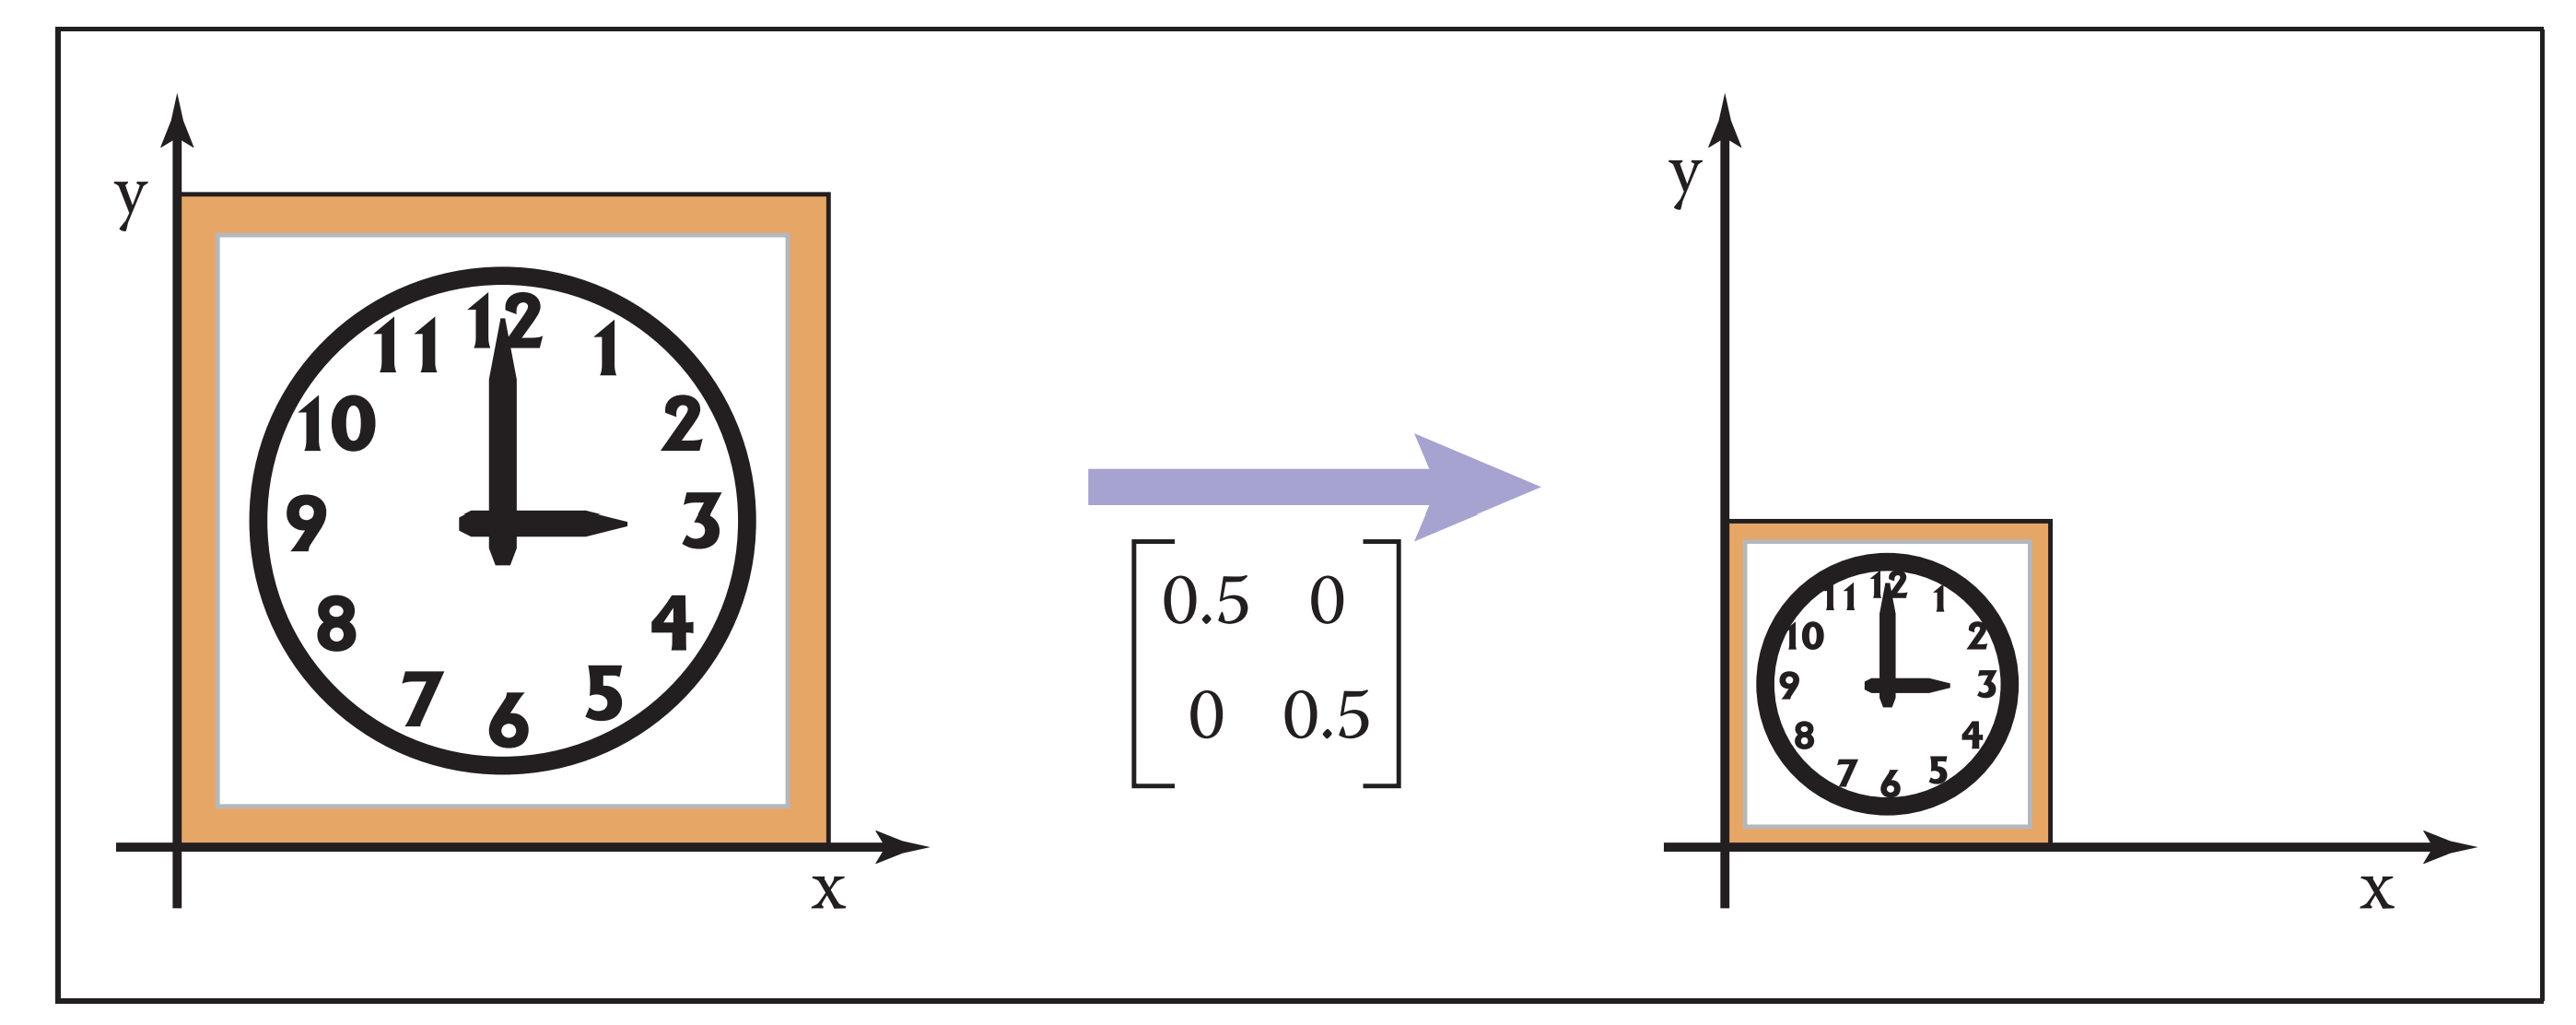
\includegraphics[scale=0.4]{Figure7.1.png}
	\caption{每个轴均匀缩放一半:轴对齐的缩放矩阵,对角线元素是缩放比例,非对角线的元素是零。}
	\label{fig:7.1}
\end{figure}

水平方向减半,垂直方向增加三倍的矩阵为(图\ref{fig:7.2}):

	\begin{equation}
		\operatorname{scale}\left(0.5, 1.5 \right)=\left[\begin{array}{cc}
			0.5 & 0 \\
			0 & 1.5
		\end{array}\right]
		\nonumber
	\end{equation}

\begin{figure}[htbp]
	\centering
	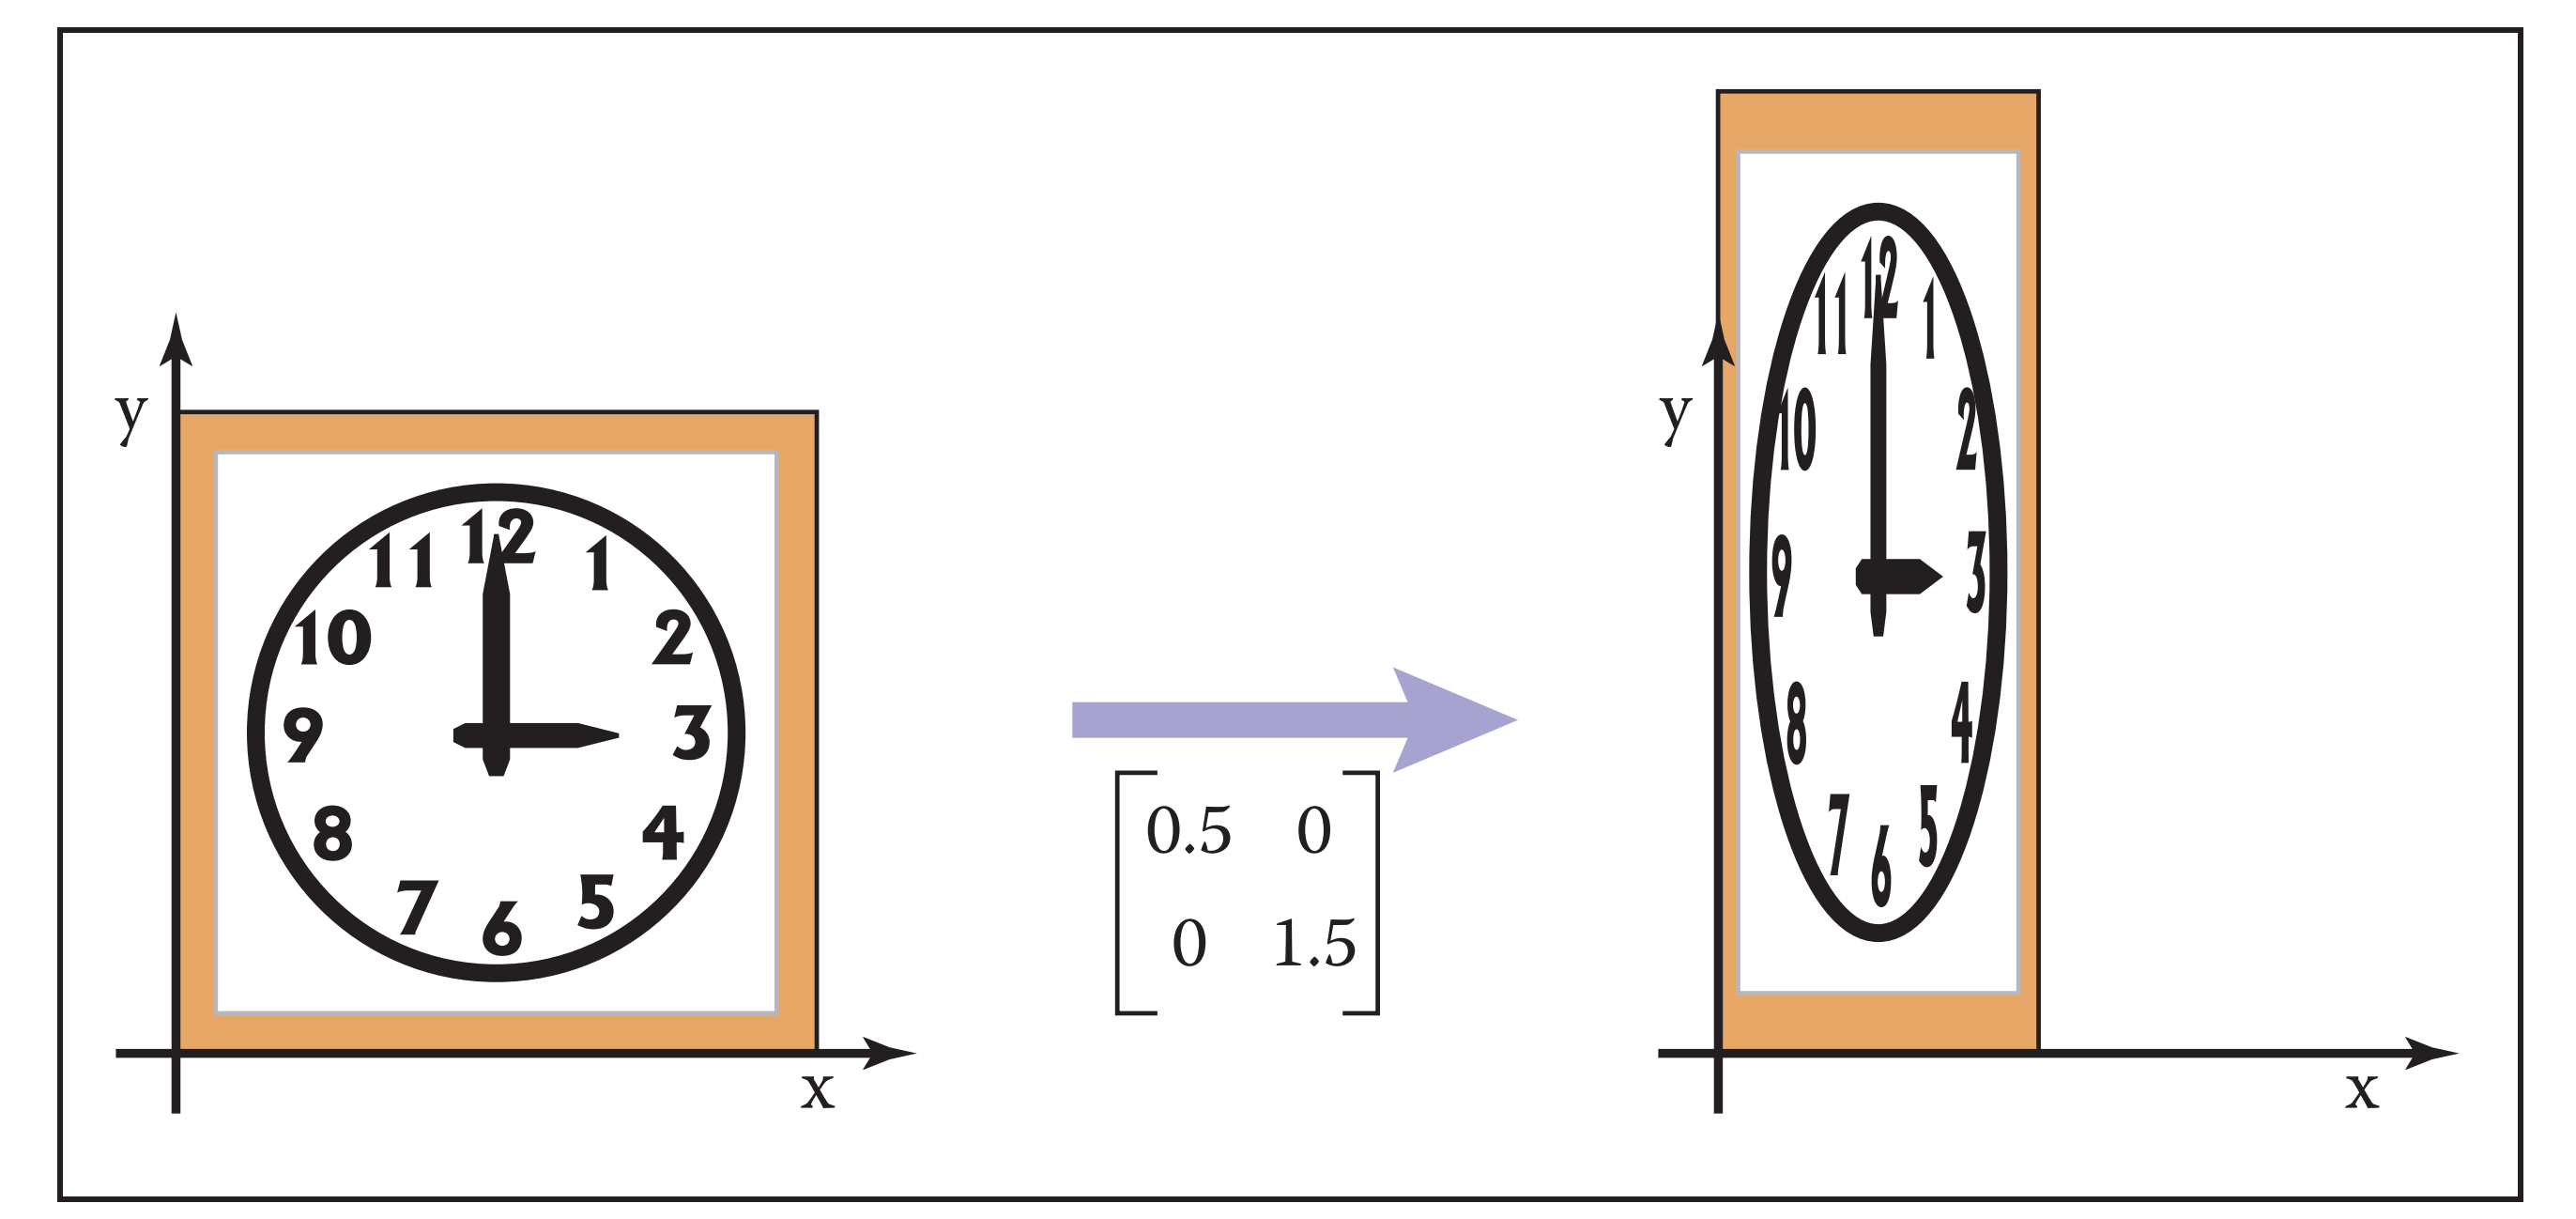
\includegraphics[scale=0.41]{Figure7.2.png}
	\caption{在x和y中不均匀缩放:缩放矩阵是对角阵,对角线元素不相等。注意到时钟的方形轮廓变为矩形,圆形则变为椭圆形。}
	\label{fig:7.2}
\end{figure}

\end{example}

\subsection{错切(Shearing)}

错切是一种将东西推向侧边,产生一种“摊牌”的效果。最下面的牌保持不动,牌越靠近牌顶,移动得越多。水平和垂直的错切矩阵是:

\begin{equation}
	\operatorname{shear-x}(s)=\left[\begin{array}{ll}
		1 & s \\
		0 & 1
	\end{array}\right], \quad \text { shear-y }(s)=\left[\begin{array}{ll}
		1 & 0 \\
		s & 1
	\end{array}\right]
\nonumber
\end{equation}

\begin{example}
	水平错切使垂直线变成向右倾斜45度线的变换是(如图\ref{fig:7.3}):
	\begin{equation}
		\operatorname{shear-x}(1)=\left[\begin{array}{ll}
			1 & 1 \\
			0 & 1
		\end{array}\right]
		\nonumber
	\end{equation}

\begin{figure}[htbp]
	\centering
	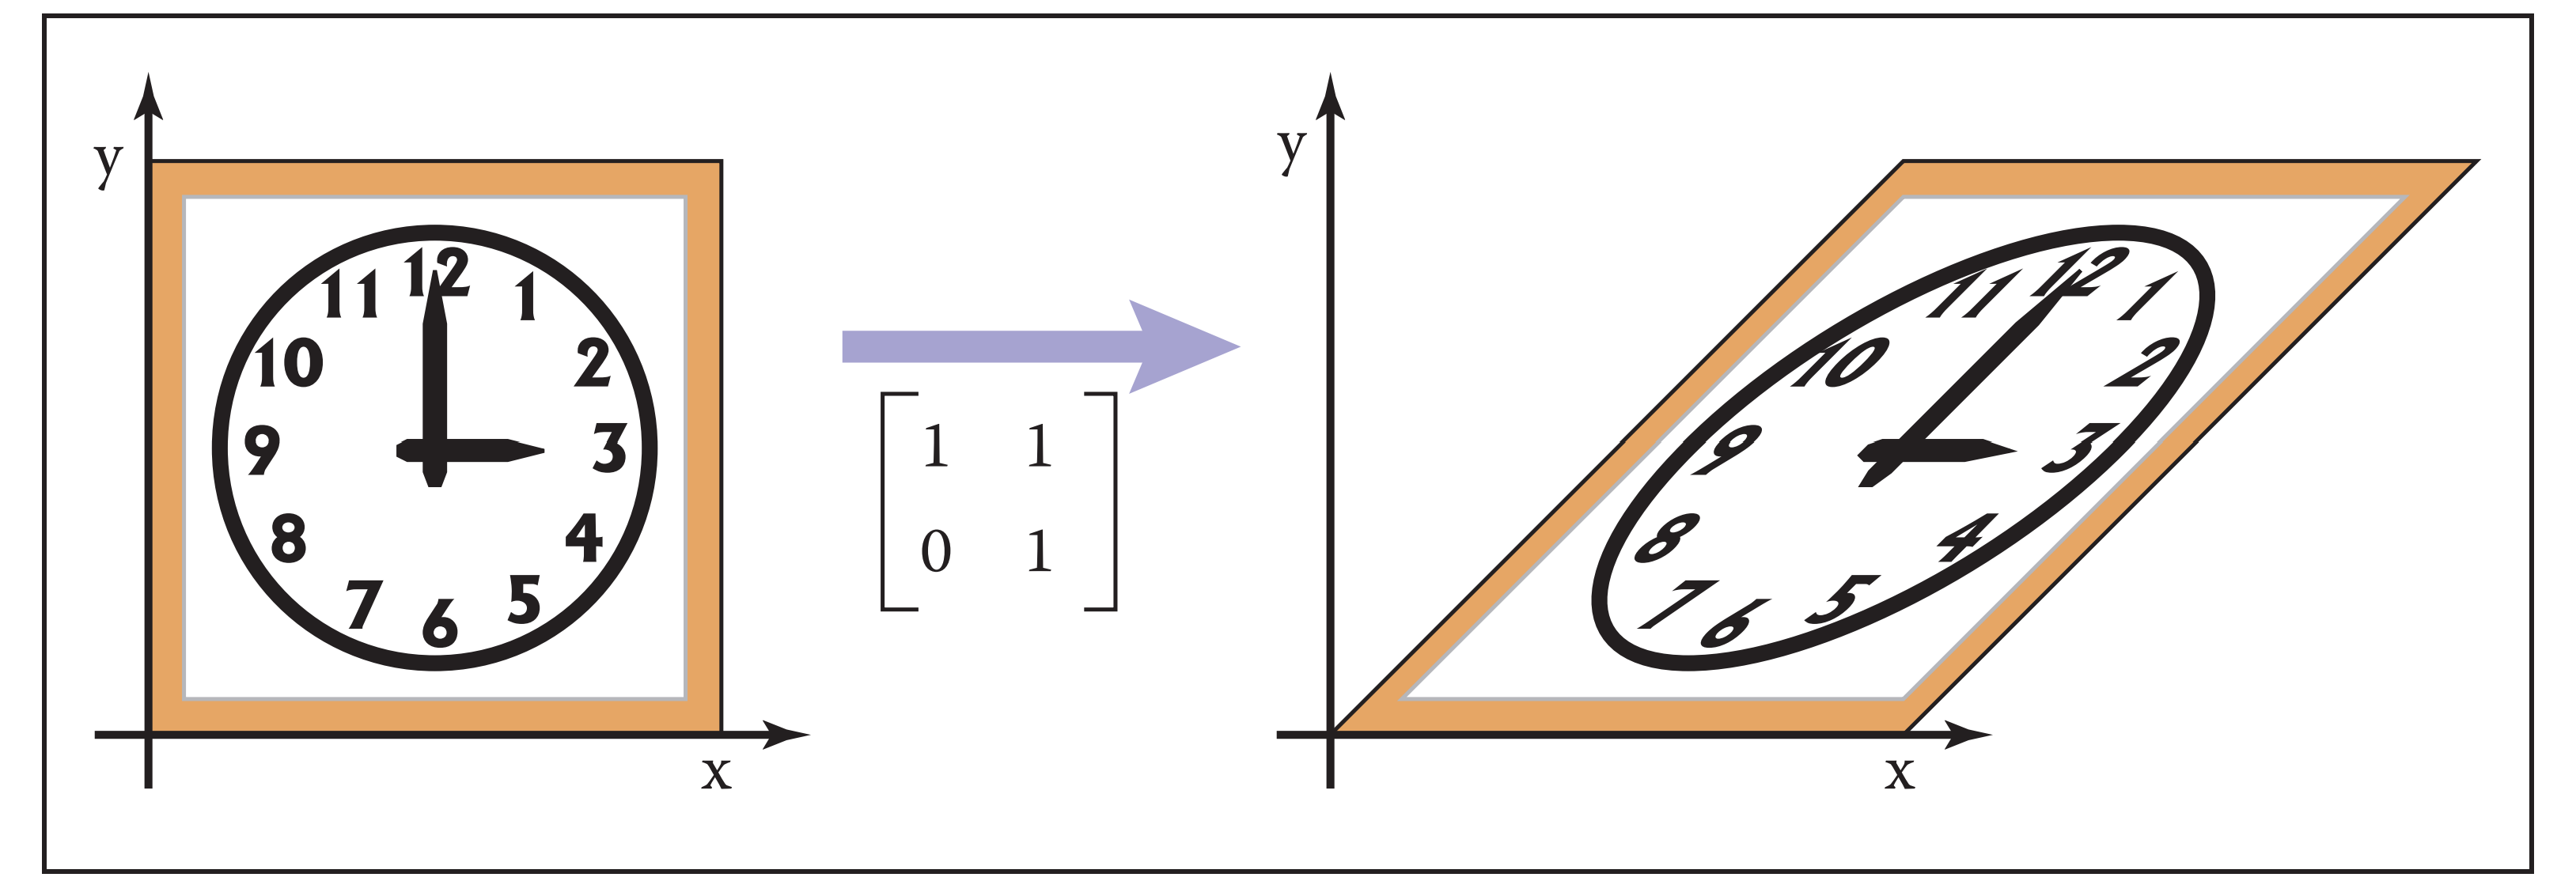
\includegraphics[scale=0.4]{Figure7.3.png}
	\caption{x错切矩阵将点向右移动,按点在y坐标位置的比例。如此,时钟的正方形轮廓变成了平行四边形,而随着缩放,时钟的圆形表面变成了椭圆。}
	\label{fig:7.3}
\end{figure}
	
\begin{figure}[htbp]
	\centering
	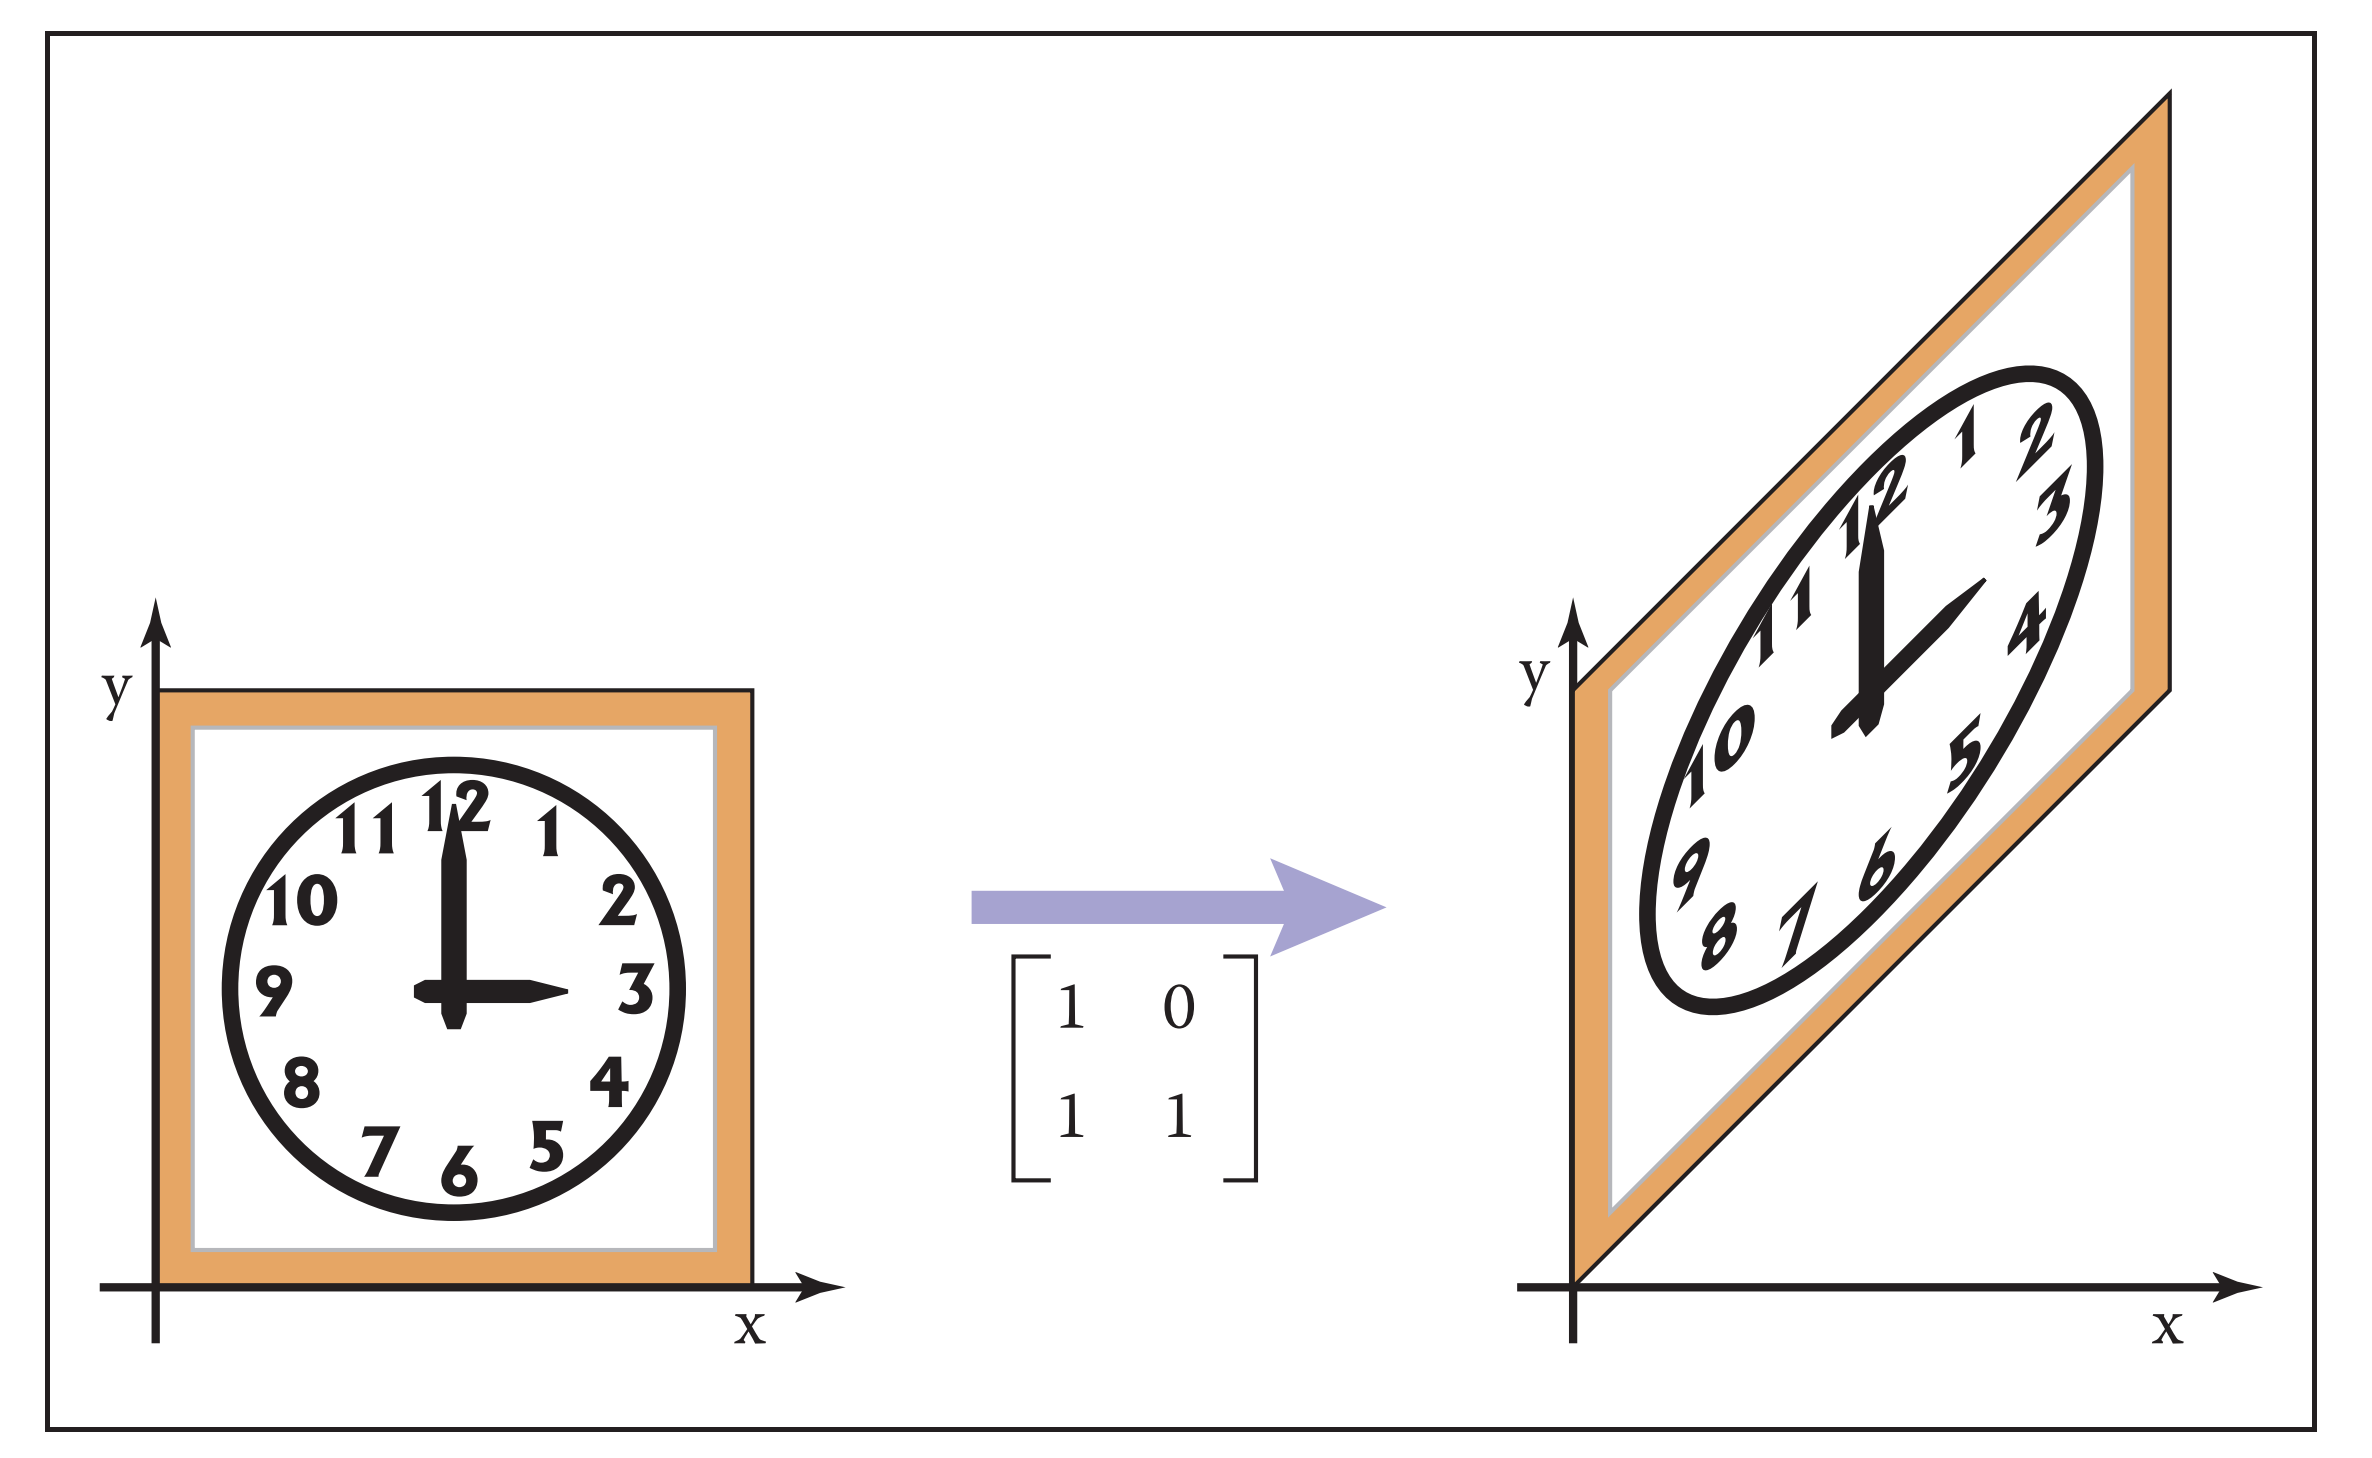
\includegraphics[scale=0.5]{Figure7.4.png}
	\caption{y错切矩阵将点向上移动,按照点在x坐标位置的比例。}
	\label{fig:7.4}
\end{figure}	
	
	垂直方向上类似的变换是(如图\ref{fig:7.4}):
	
	\begin{equation}
		\operatorname{shear-y}(1)=\left[\begin{array}{ll}
			1 & 0 \\
			1 & 1
		\end{array}\right]
		\nonumber
	\end{equation}
	
	在这两种情况下,时钟的正方形轮廓变成平行四边形,而时钟的圆形表盘外轮廓变成椭圆形\footnote{事实上,任何矩阵变换下的圆的图像都是椭圆。}。
	
	另一种考虑错切的方式是仅考虑垂直(或水平)轴的旋转。取垂直轴并顺时针倾斜角度$\phi$的错切变换为:
	
	\begin{equation}
		\left[\begin{array}{ll}
			1 &  \rm tan \phi \\
			0 & 1
		\end{array}\right]
		\nonumber
	\end{equation}

	类似地,将水平轴逆时针旋转角度$\phi$的错切矩阵为:
	
	\begin{equation}
		\left[\begin{array}{ll}
			1 &  0 \\
			\rm tan \phi & 1
		\end{array}\right]
		\nonumber
	\end{equation}
	
\end{example}

\subsection{旋转(Rotation)}

假设我们想逆时针旋转向量$\mathbf{a}$一个角度$\phi$,得到向量$\mathbf{b}$(如图\ref{fig:7.5})。如果$\mathbf{a}$与$x$轴成角度$\alpha$,其长度为$r=\sqrt{x_a^2+y_a^2}$,那么我们知道:

\begin{equation}
	\begin{aligned}
		& x_a=r \cos \alpha \\
		& y_a=r \sin \alpha
	\end{aligned}
\nonumber
\end{equation}

\begin{figure}[htbp]
	\centering
	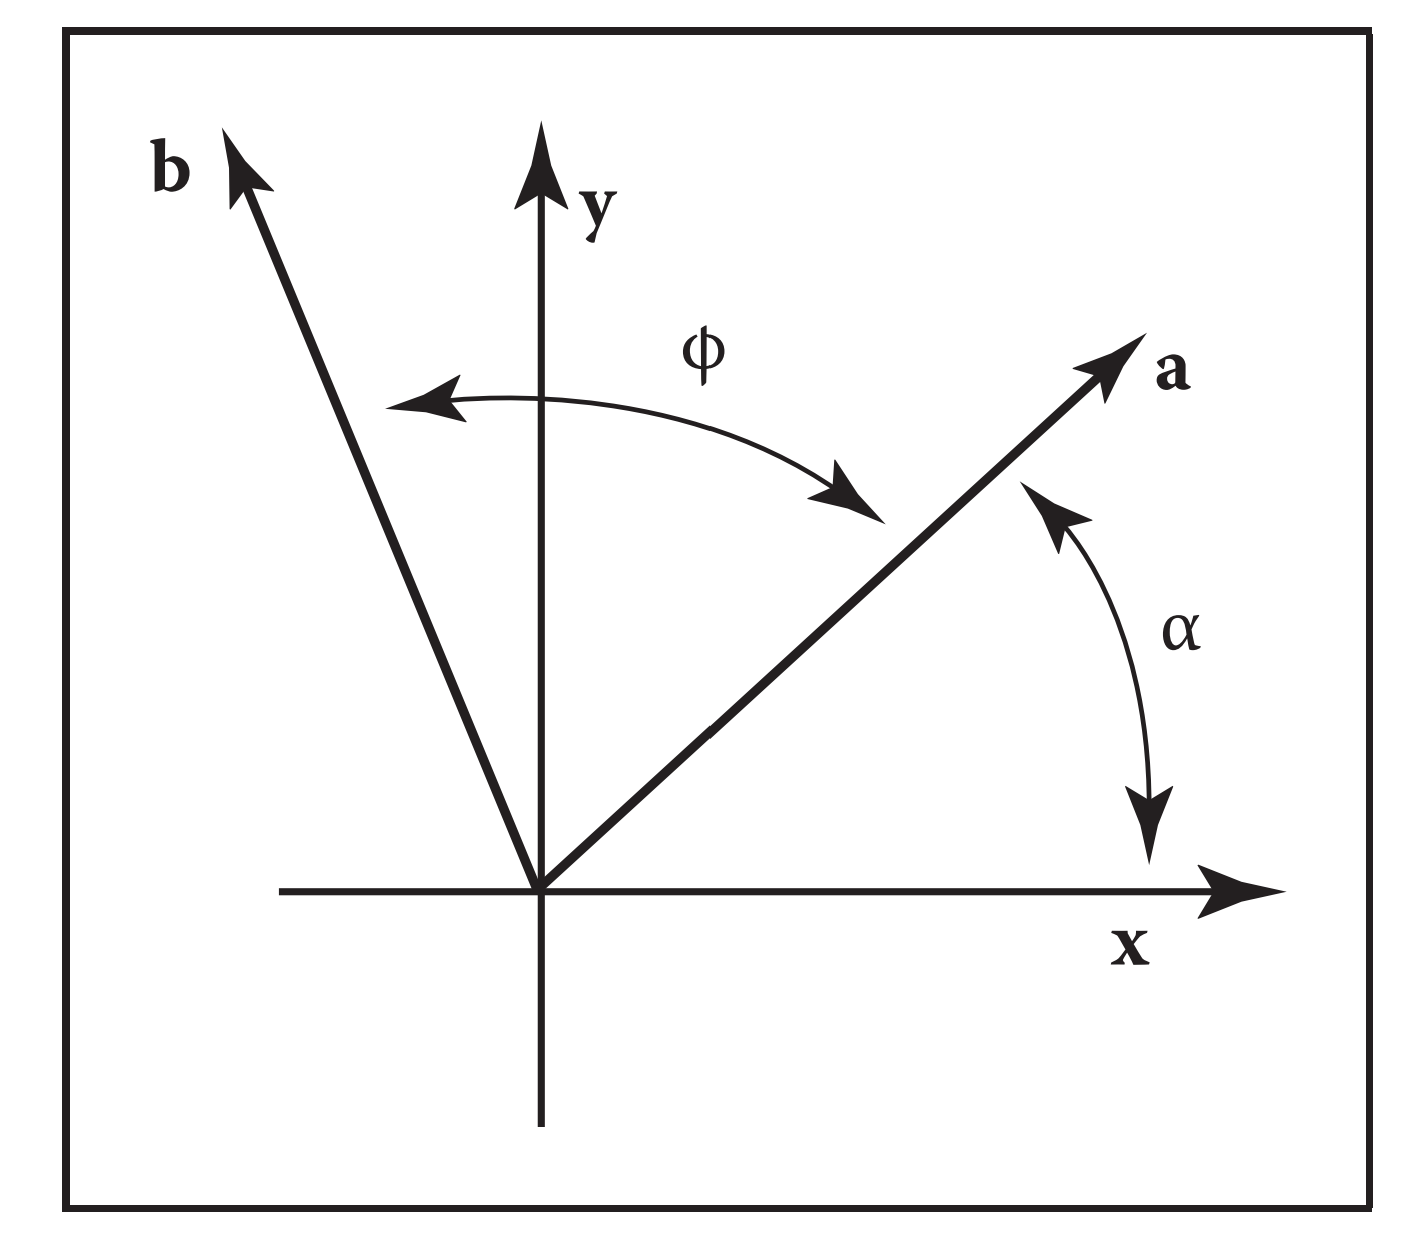
\includegraphics[scale=0.4]{Figure7.5.png}
	\caption{方程\ref{con:7.1}的几何图示}
	\label{fig:7.5}
\end{figure}	

因为$\mathbf{b}$是$\mathbf{a}$旋转而来,所以$\mathbf{b}$的长度也是$r$。$\mathbf{b}$是$\mathbf{a}$旋转$\phi$角度,所以$\mathbf{b}$与$x$轴之间的夹角是$(\alpha + \phi)$。使用三角加法恒等式(第\ref{label}小节):

\begin{equation}\label{con:7.1}
	\begin{aligned}
		& x_b=r \cos (\alpha+\phi)= r \cos \alpha \cos \phi-r \sin \alpha \sin \phi \\
		& y_b=r \sin (\alpha+\phi)= r \sin \alpha \cos \phi+r \cos \alpha \sin \phi
	\end{aligned}
\end{equation}

将$\mathbf{a}$向量带入式\ref{con:7.1},$x_a=r \cos \alpha$,$y_a=r \sin \alpha$,故可以得到:

\begin{equation}
	\begin{aligned}
		 x_b &= x_a \cos \phi - y_a \sin \phi \\
		 y_b &= y_a \cos \phi + x_a \sin \phi
	\end{aligned}
\nonumber
\end{equation}

所以从$\mathbf{a}$变换到$\mathbf{b}$的矩阵形式为:

\begin{equation}
	\operatorname{rotate}(\phi)=\left[\begin{array}{rr}
		\cos \phi & -\sin \phi \\
		\sin \phi & \cos \phi
	\end{array}\right]
\nonumber
\end{equation}

\begin{example}
	旋转$pi / 4$弧度($45^{\circ}$)的旋转矩阵是(如图\ref{fig:7.6}):
	\begin{equation}
		\left[\begin{array}{cr}
			\cos \frac{\pi}{4} & -\sin \frac{\pi}{4} \\
			\sin \frac{\pi}{4} & \cos \frac{\pi}{4}
		\end{array}\right]=\left[\begin{array}{rr}
			0.707 & -0.707 \\
			0.707 & 0.707
		\end{array}\right] \text {. }
	\end{equation}
	
	\begin{figure}[htbp]
		\centering
		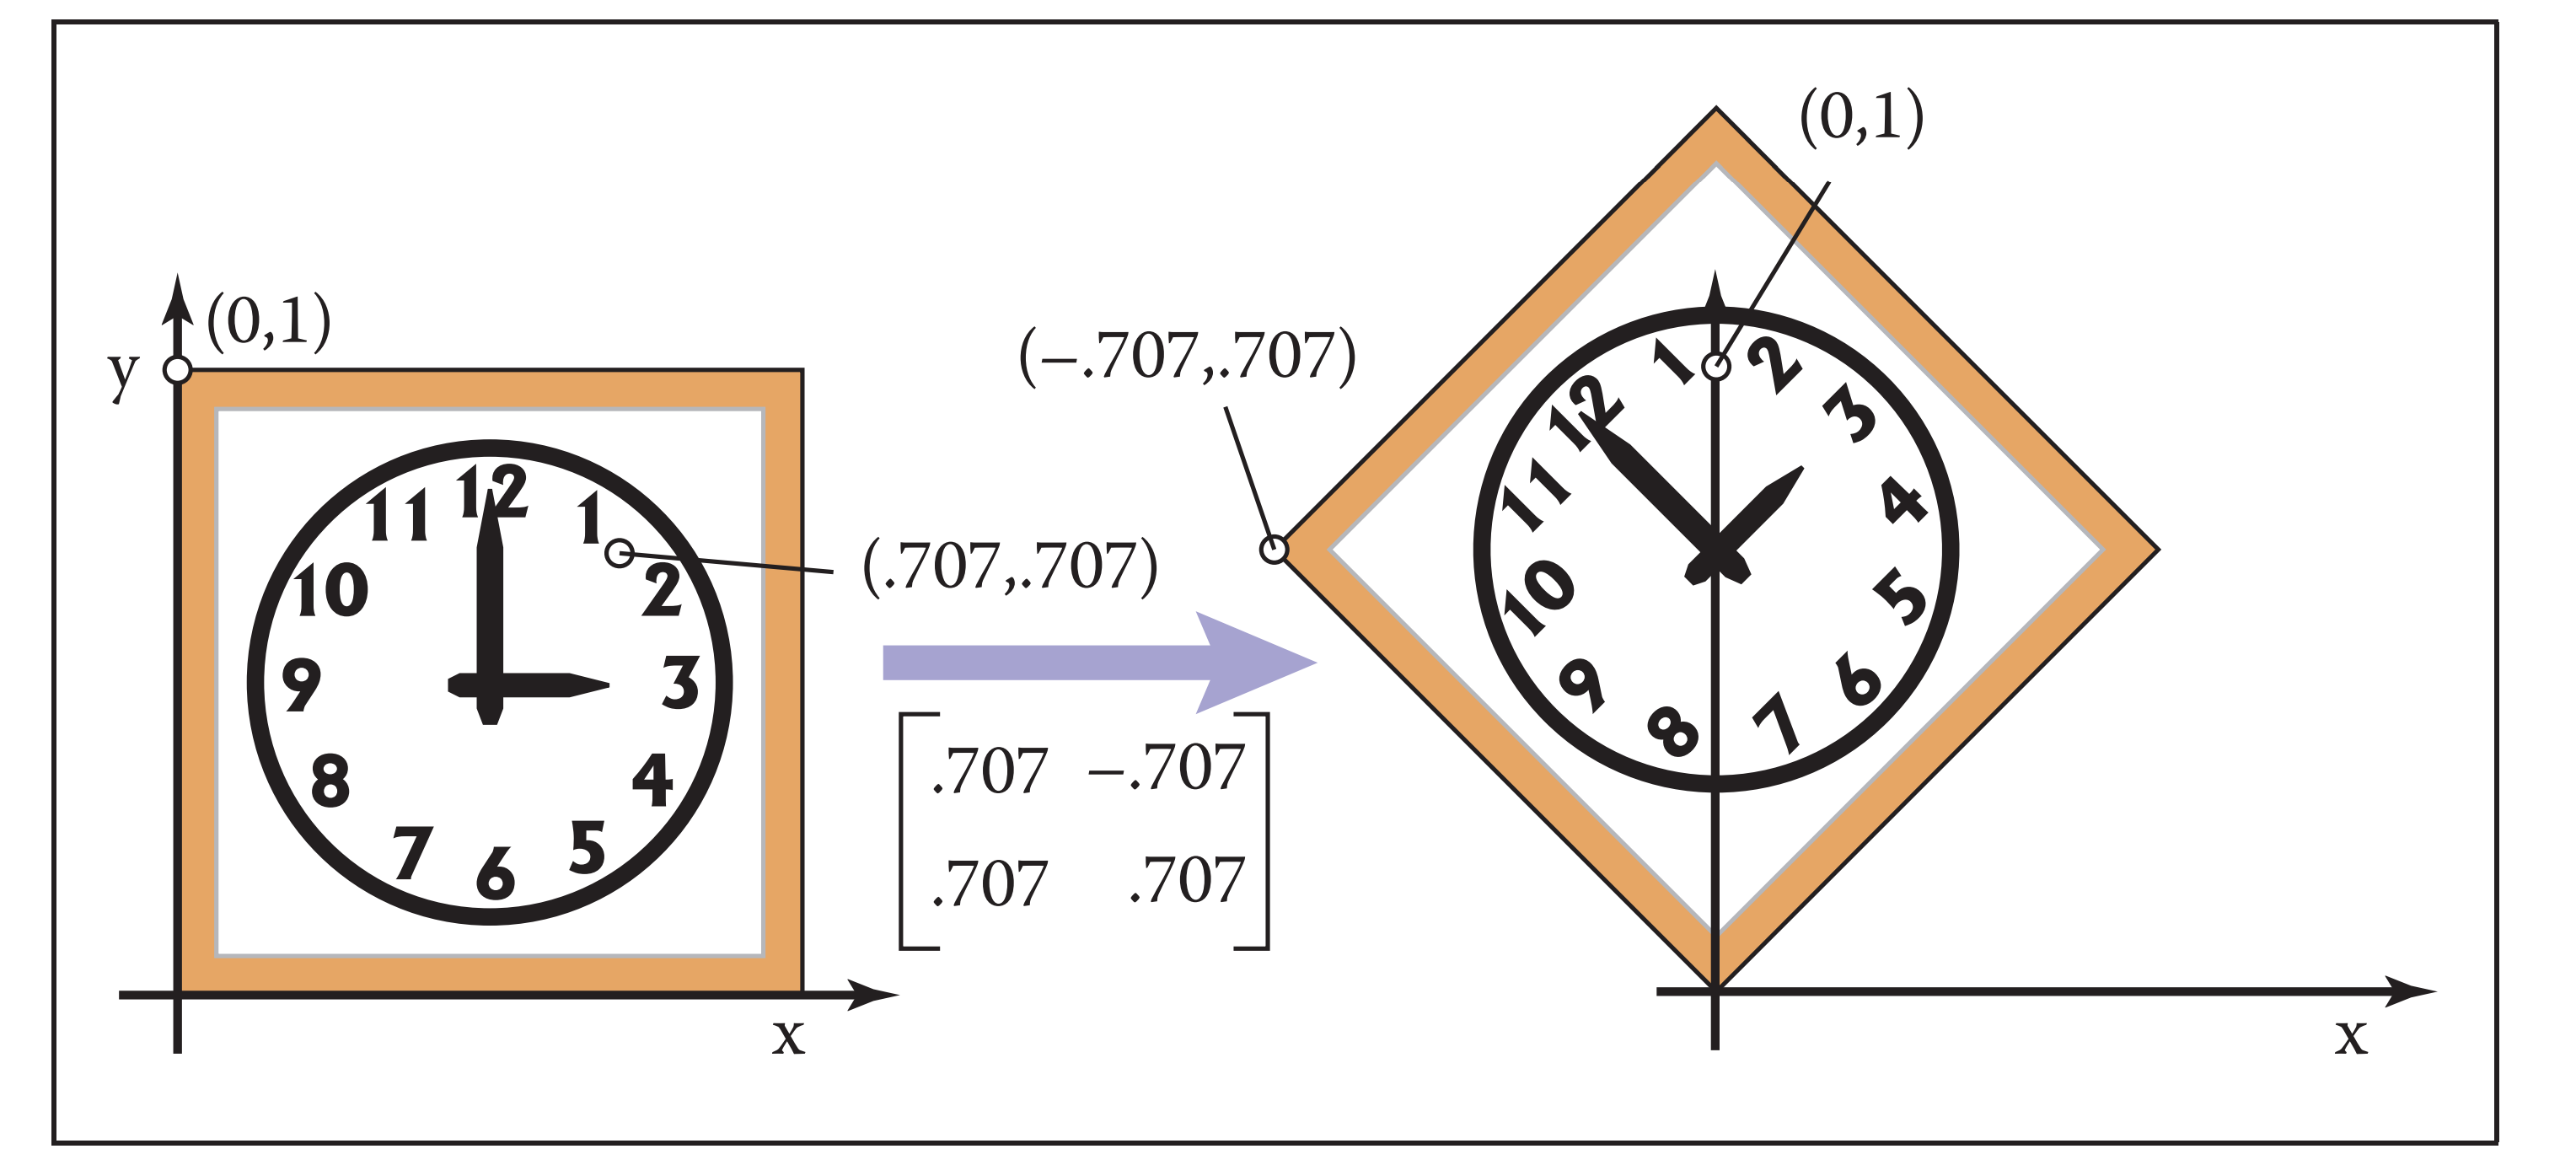
\includegraphics[scale=0.4]{Figure7.6.png}
		\caption{旋转$45^{\circ}$。注意到旋转是逆时针的,$cos(45^{\circ}) = sin(45^{\circ}) \approx .707 $}
		\label{fig:7.6}
	\end{figure}	
	
	顺时针方向旋转$\pi / 6$弧度($30^{\circ}$),在我们的框架中是旋转$-\pi / 6$弧度的旋转矩阵(如图\ref{fig:7.7}):
	
	\begin{equation}
		\left[\begin{array}{cr}
			\cos \frac{-\pi}{6} & -\sin \frac{-\pi}{6} \\
			\sin \frac{-\pi}{6} & \cos \frac{-\pi}{6}
		\end{array}\right]=\left[\begin{array}{rr}
			0.866 & 0.5 \\
			-0.5 & 0.866
		\end{array}\right] \text {. }
	\end{equation}
	
	\begin{figure}[htbp]
		\centering
		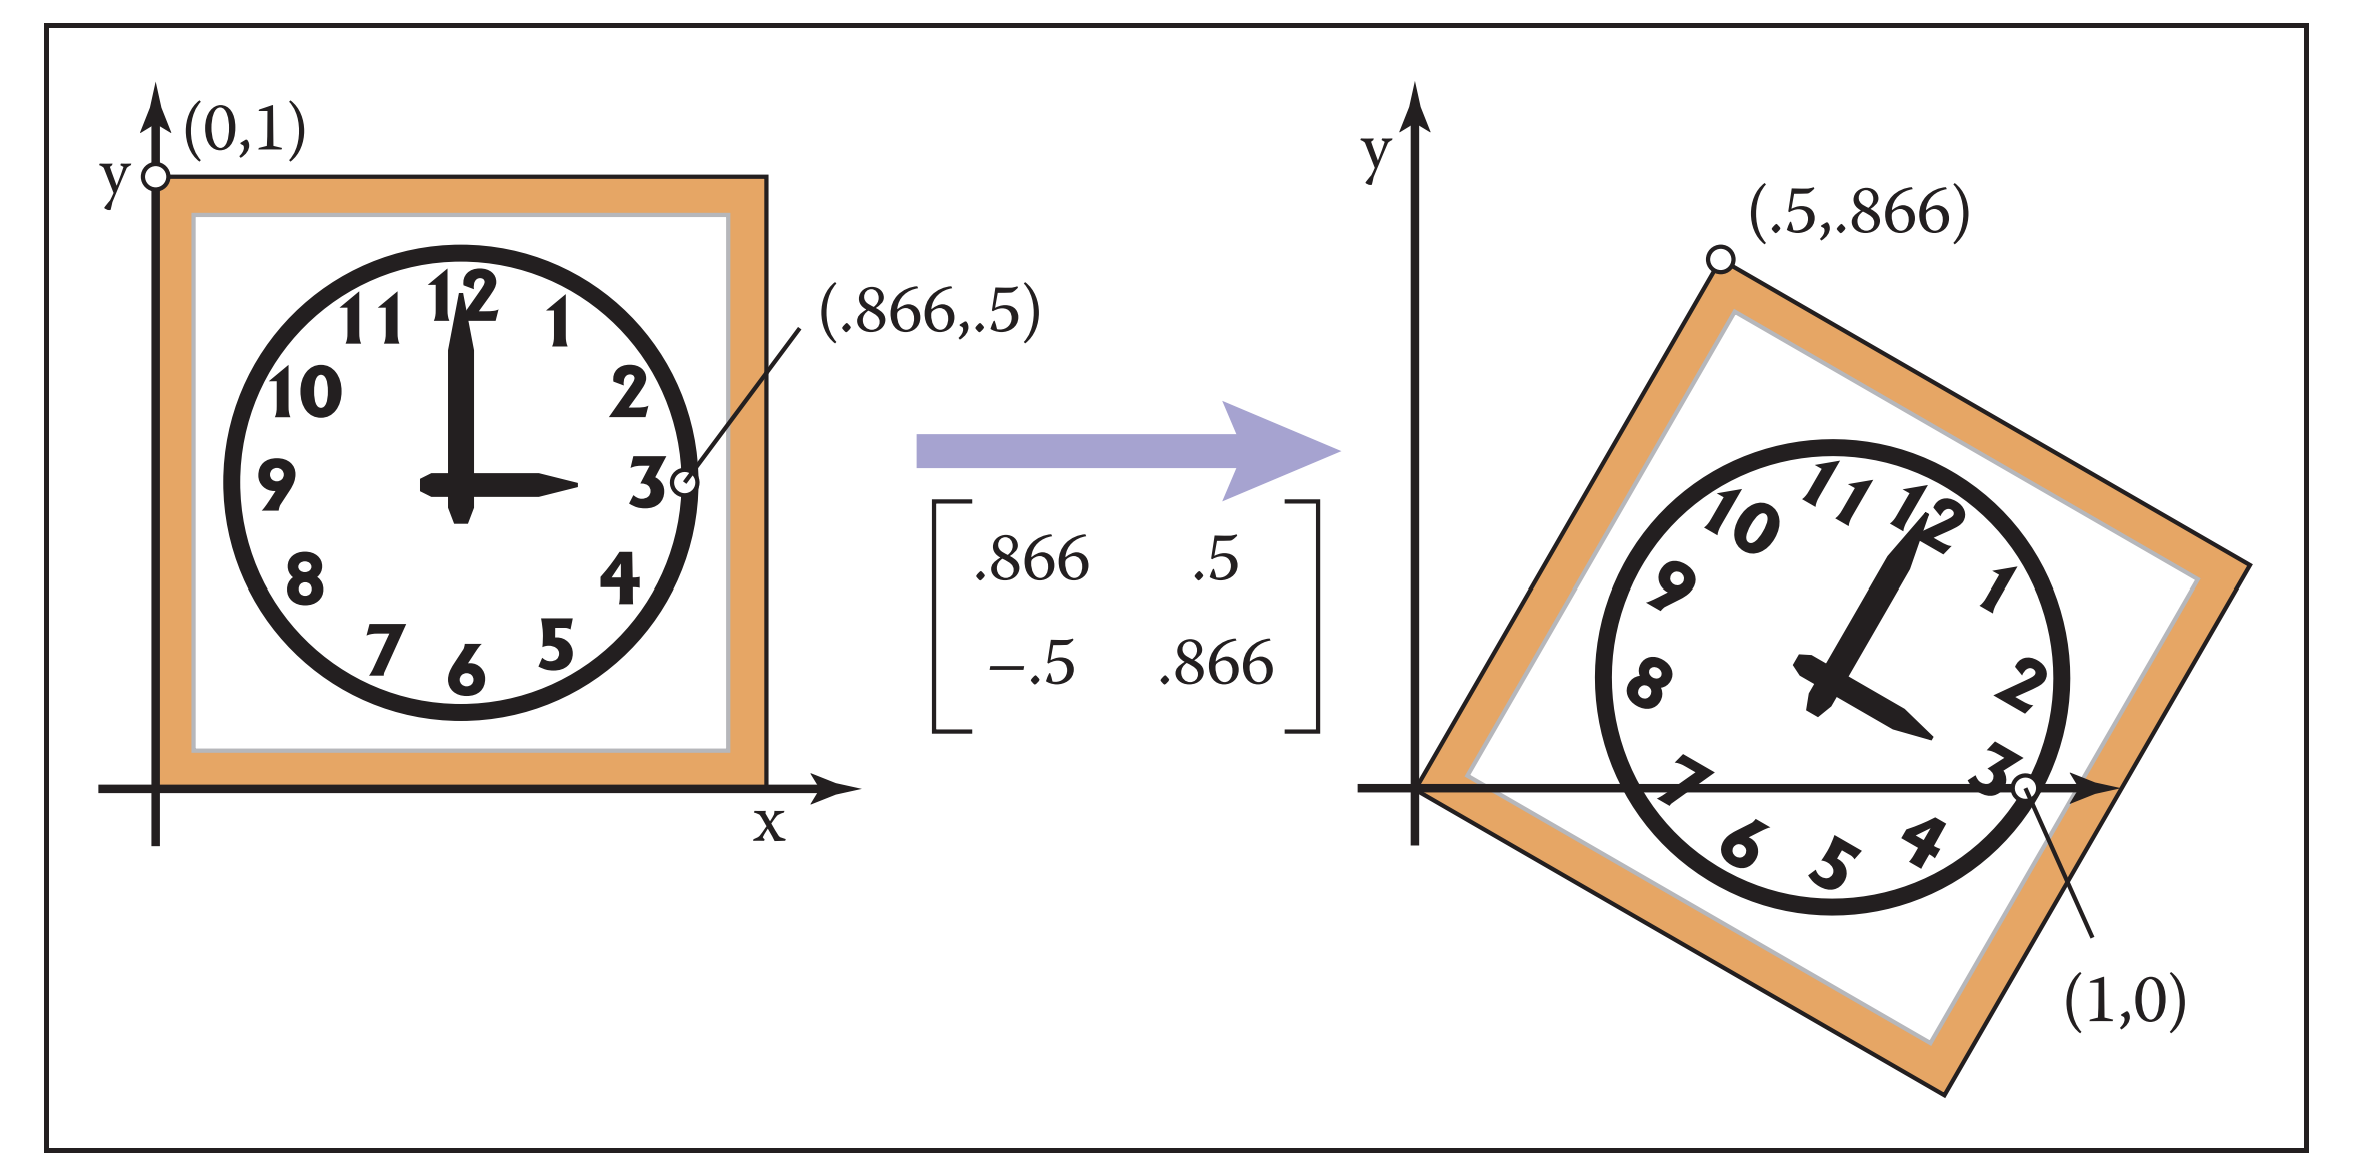
\includegraphics[scale=0.5]{Figure7.7.png}
		\caption{旋转$-30^{\circ}$。注意到旋转方向为顺时针,$cos(-30^{\circ}) \approx .866 $和$sin(-30^{\circ}) \approx -.5 $。}
		\label{fig:7.7}
	\end{figure}	
	
	
\end{example}

因为旋转矩阵每一行的范数是1$\left(\sin ^2 \phi+\cos ^2 \phi=1\right)$,并且行是正交的$(\cos \phi(-\sin \phi)+\sin \phi \cos \phi=0)$,我们看到旋转矩阵是正交矩阵(第\ref{5.2.4}节)。观察矩阵我们可以读出两对正交向量:两个列向量,(没看懂。。。)

\subsection{反射(Reflection)}

我们可以通过使用有一个负比例因子的比例矩阵来反射任一坐标轴上的向量(如图\ref{fig:7.8},图\ref{fig:7.9}):

\begin{equation}
	\text { reflect-y }=\left[\begin{array}{rr}
		-1 & 0 \\
		0 & 1
	\end{array}\right], \quad \text { reflect-x }=\left[\begin{array}{rr}
		1 & 0 \\
		0 & -1
	\end{array}\right]
\nonumber
\end{equation}

\begin{figure}[htbp]
	\centering
	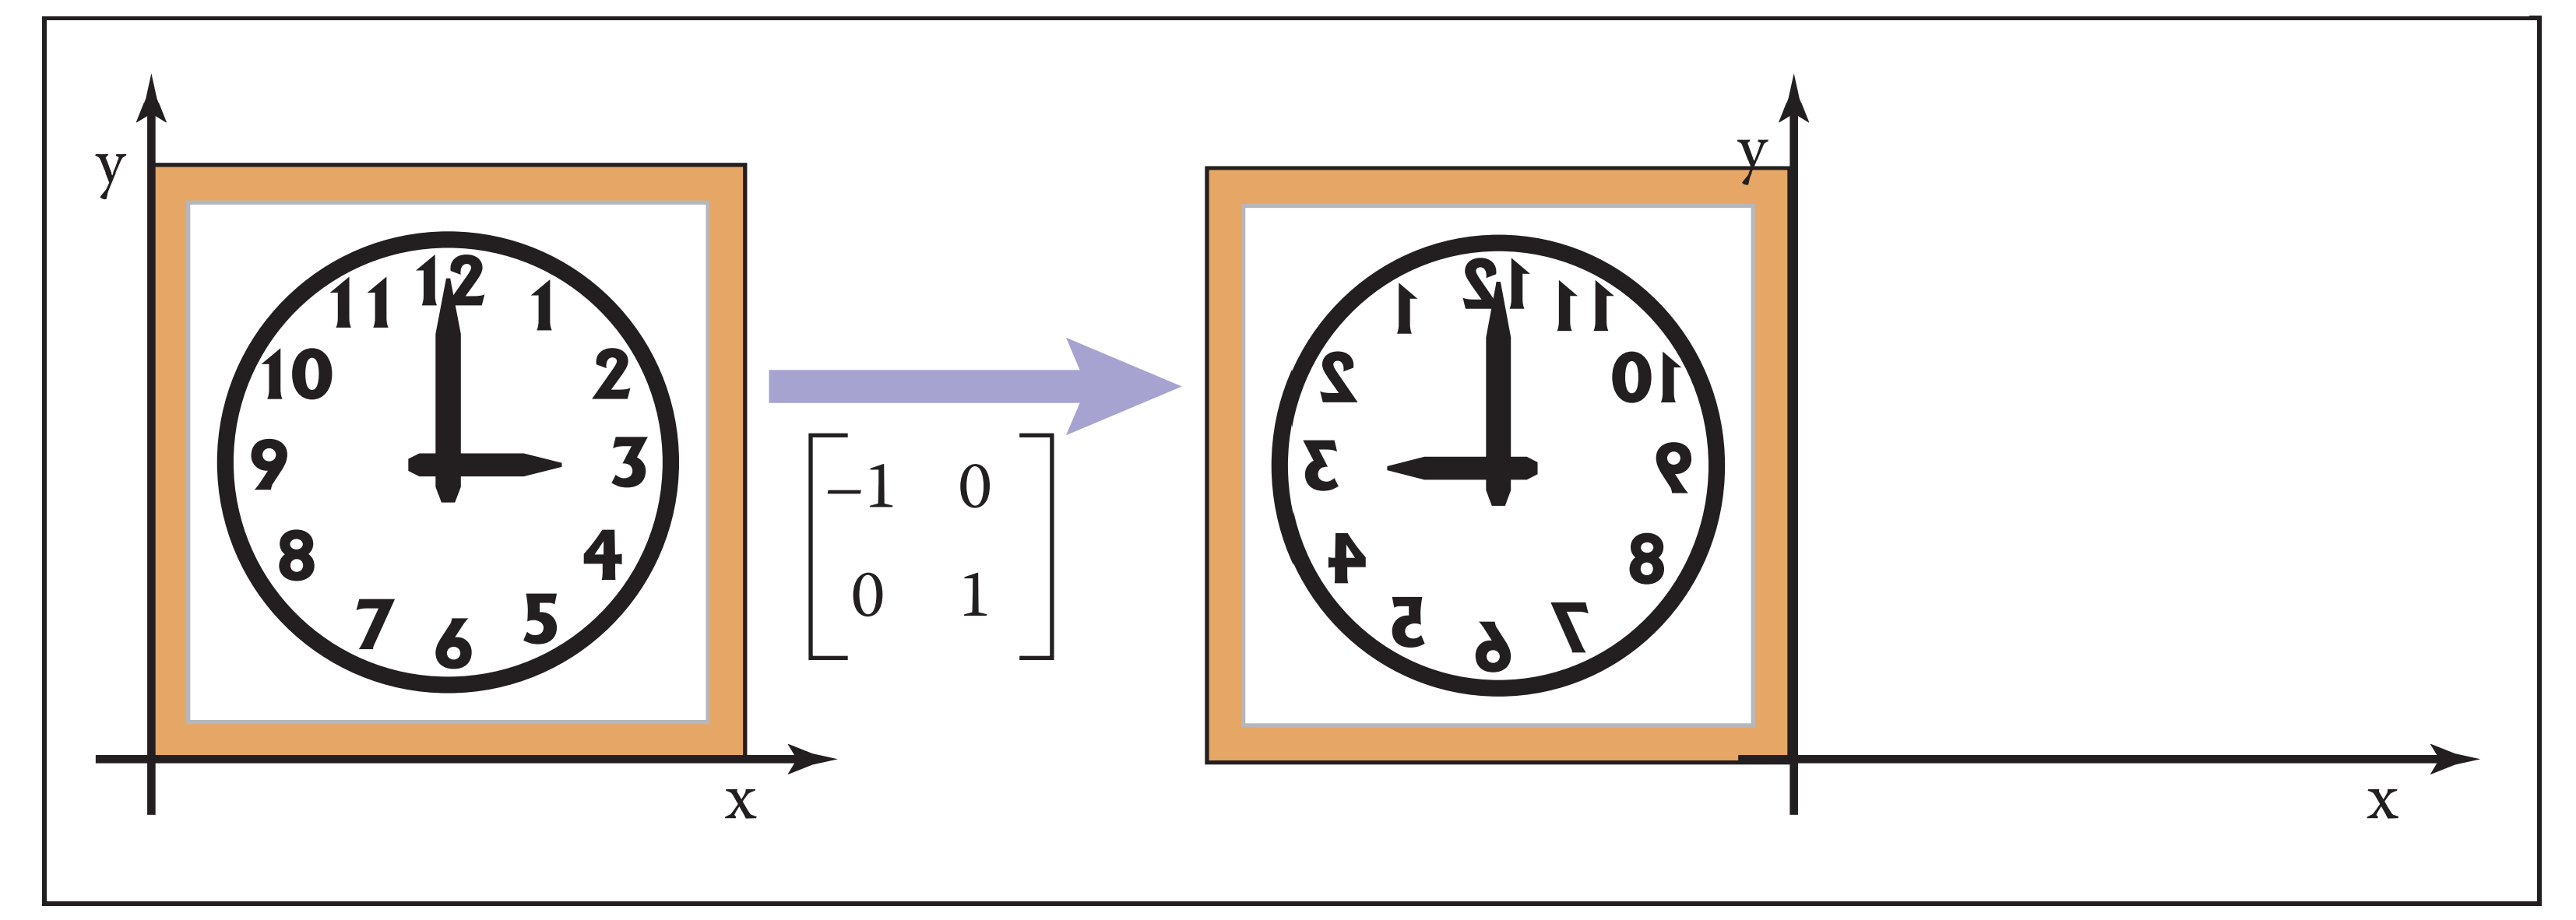
\includegraphics[scale=0.4]{Figure7.8.png}
	\caption{通过将所有x坐标乘以–1来实现关于y轴的反射。}
	\label{fig:7.8}
\end{figure}	

\begin{figure}[htbp]
	\centering
	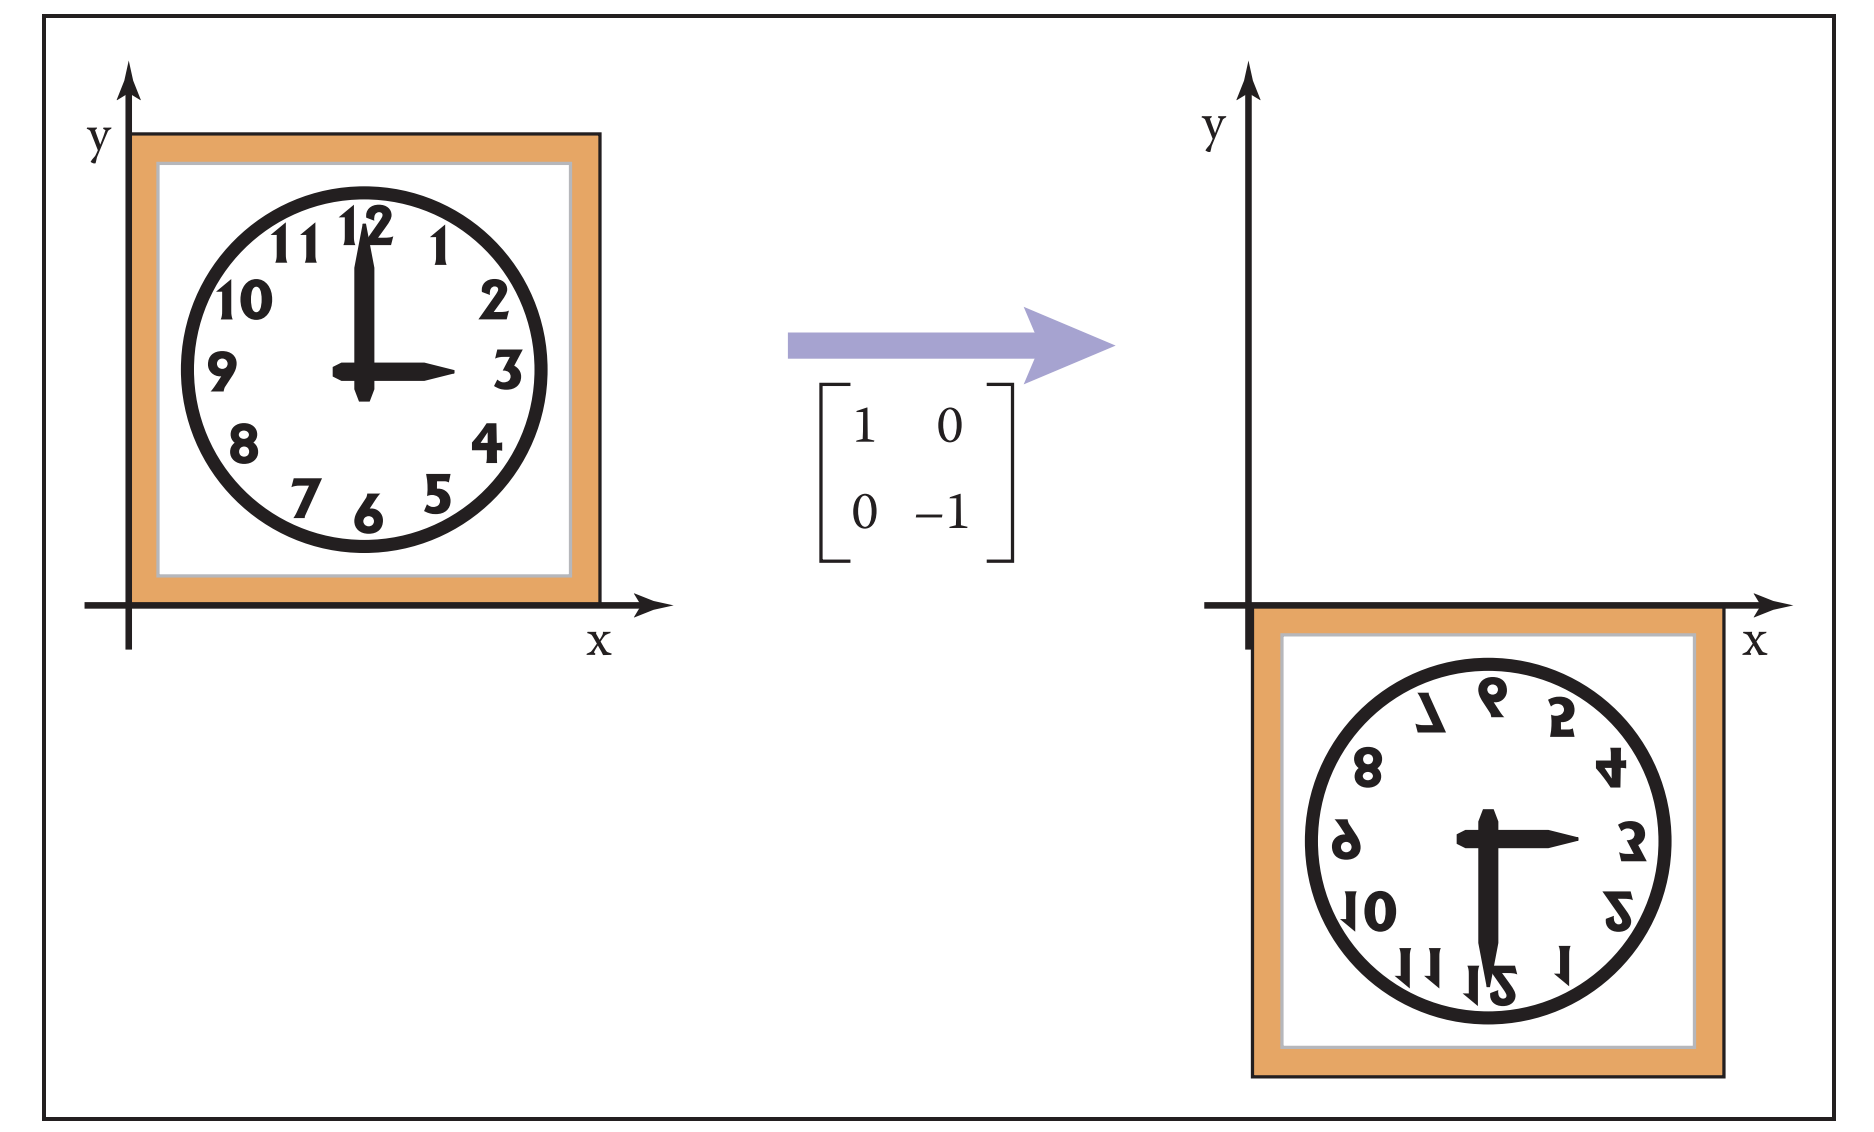
\includegraphics[scale=0.4]{Figure7.9.png}
	\caption{通过将所有y坐标乘以–1来实现关于x轴的反射。}
	\label{fig:7.9}
\end{figure}	

虽然人们可能会认为对角线的两个元素中都是−1的矩阵也是反射,但实际上它只是$\pi$弧度的旋转。

\subsection{变换的组成和分解(Composition and Decomposition of Transformations)}

图形程序通常对一个物体应用多个变换。例如,我们可能想先使用$\mathbf{S}$进行缩放,然后使用$\mathbf{R}$进行旋转。这将在二维向量$\mathbf{v}_{1}$上分两步完成:

\begin{equation}
	\text { first, } \mathbf{v}_2=\mathbf{S} \mathbf{v}_1, \text { then, } \mathbf{v}_3=\mathbf{R v}_2
	\nonumber
\end{equation}

另一种书写方式为:

\begin{equation}
	\mathbf{v}_3=\mathbf{R}\left(\mathbf{S v}_1\right)
	\nonumber
\end{equation}

因为矩阵乘法是满足结合律的,所以我们也可以写为:

\begin{equation}
	\mathbf{v}_3=(\mathbf{R S}) \mathbf{v}_1
	\nonumber
\end{equation}

换言之,我们可以使用相同大小的单个矩阵来表示由两个矩阵对向量变换的效果,我们可以将两个矩阵相乘来得到这个矩阵:$\mathbf{M}=\mathbf{R S}$(如图\ref{fig:7.10})。

请记住这些变换是从右侧进行变换的,这非常重要。所以矩阵$\mathbf{M}=\mathbf{R S}$先应用$\mathbf{S}$后应用$\mathbf{R}$。

\begin{figure}[htbp]
	\centering
	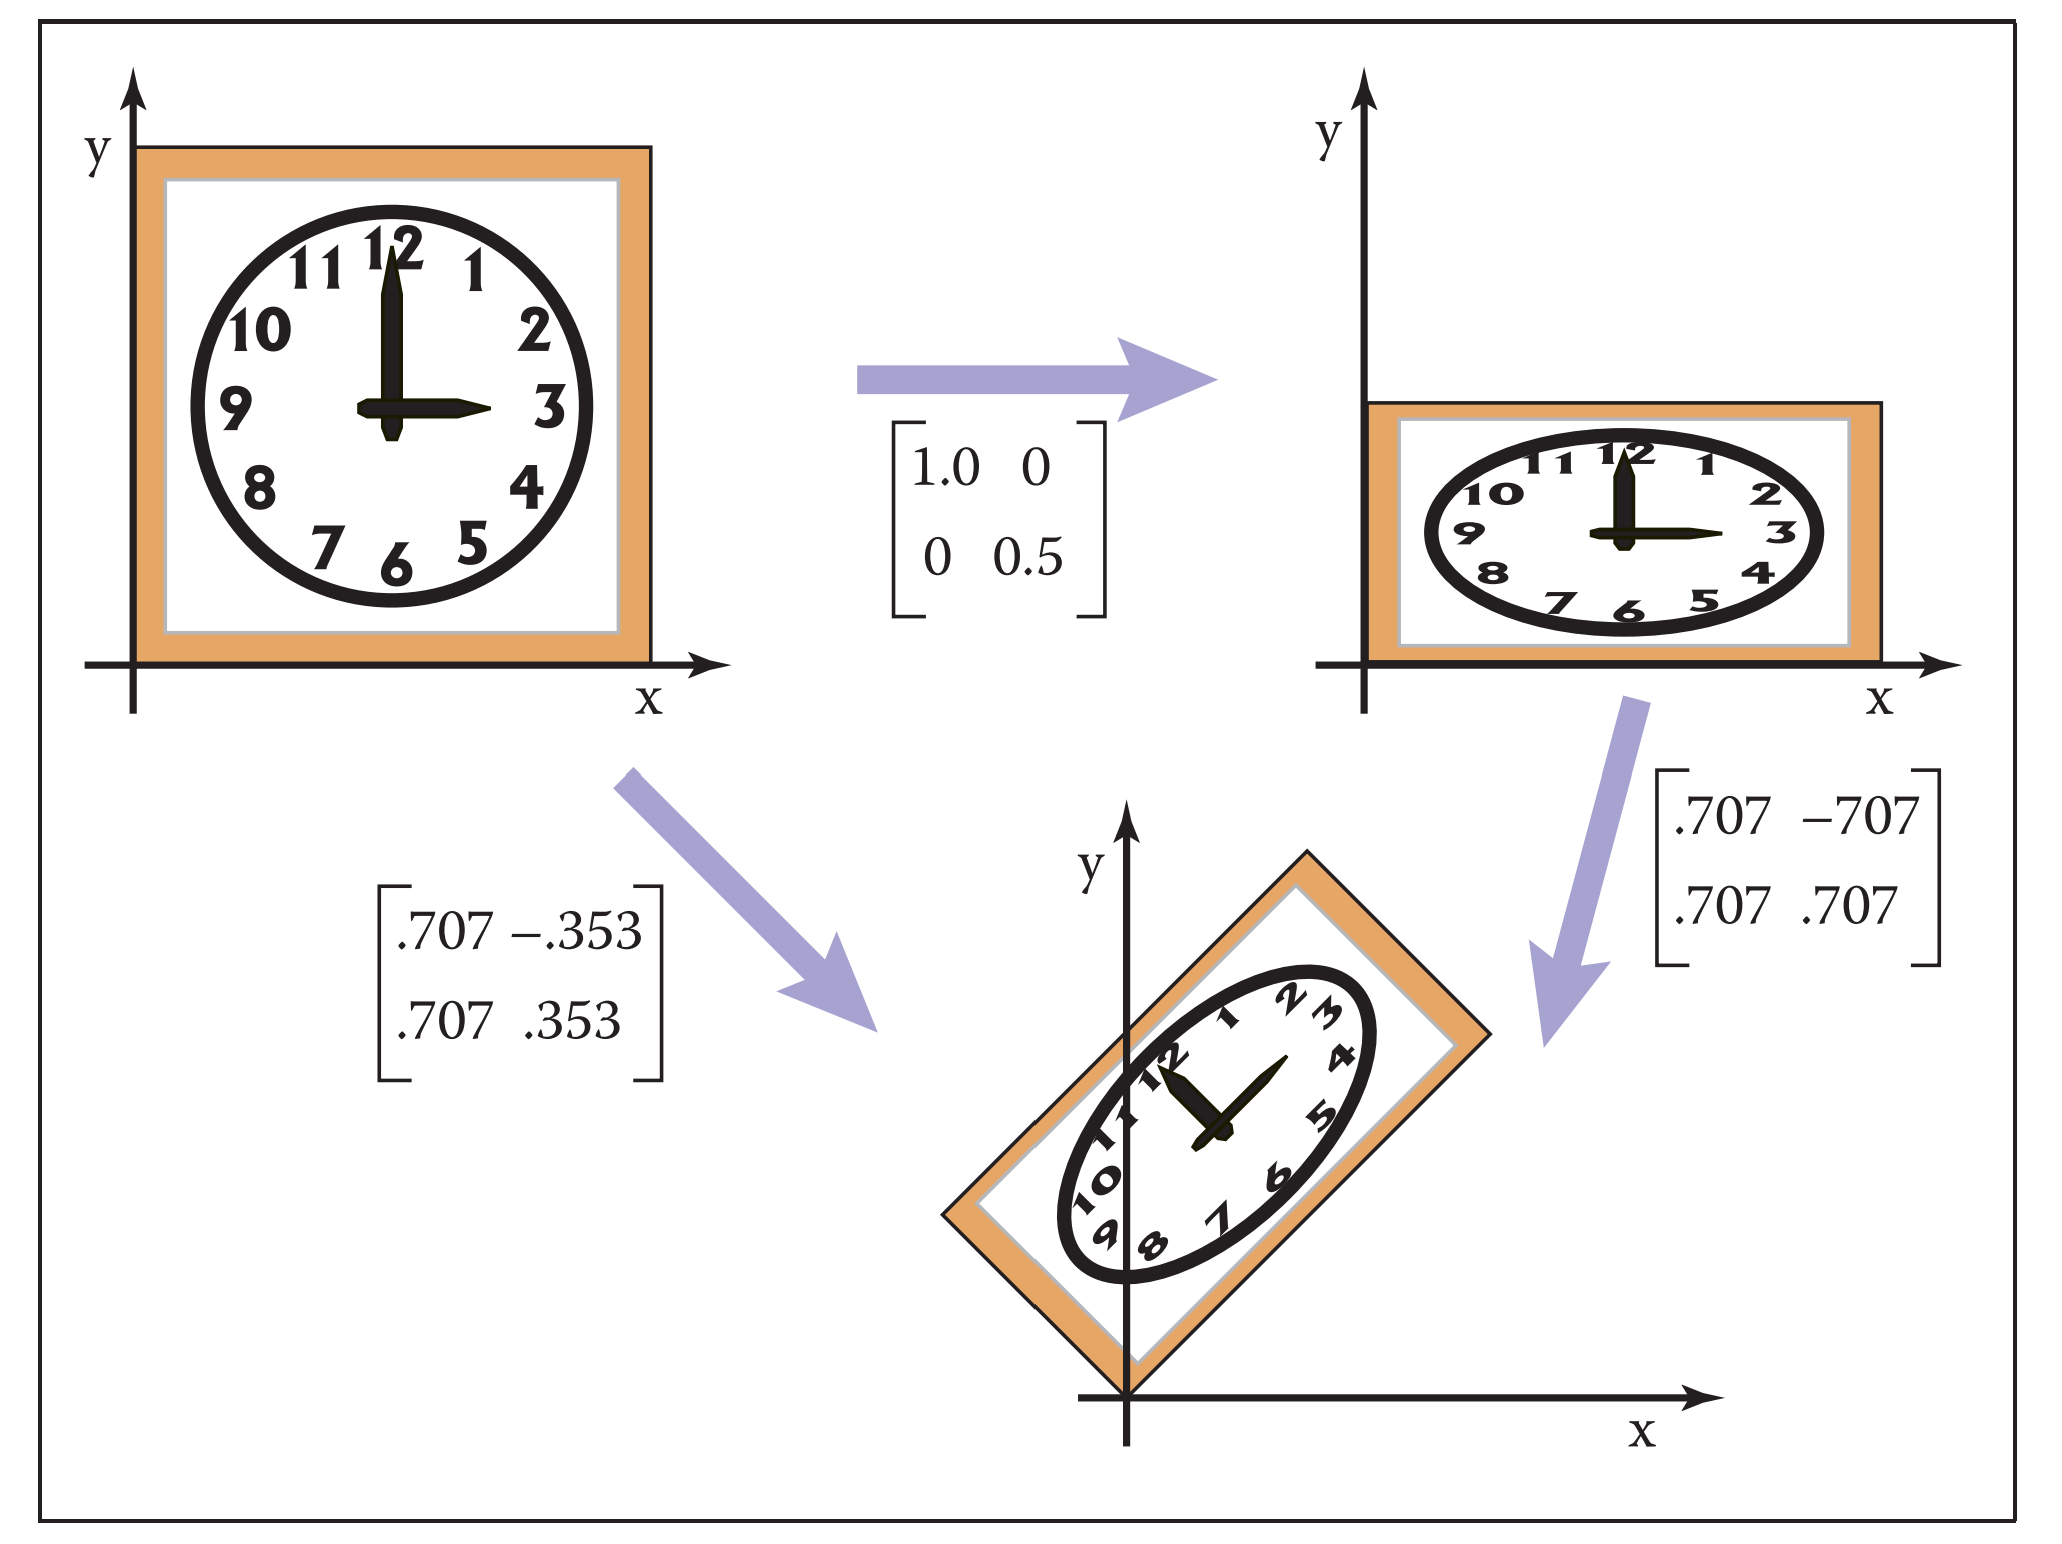
\includegraphics[scale=0.4]{Figure7.10.png}
	\caption{依次应用两个变换矩阵与应用一次这些矩阵的乘积是一样的。这是一个十分关键的概念,是大多数图形硬件和软件的基础。}
	\label{fig:7.10}
\end{figure}	

\begin{example}
	假设我们想在垂直方向上缩放一半,然后旋转$\pi/4$弧度($45^{\circ}$),其变换矩阵为:
	
	\begin{equation}
		\left[\begin{array}{cr}
			0.707 & -0.707 \\
			0.707 & 0.707
		\end{array}\right]\left[\begin{array}{cc}
			1 & 0 \\
			0 & 0.5
		\end{array}\right]=\left[\begin{array}{cc}
			0.707 & -0.353 \\
			0.707 & 0.353
		\end{array}\right]
	\nonumber
	\end{equation}

请务必记住矩阵乘法不是可交换的。所以变换的顺序很重要。对于这个例子,先进行旋转再进行缩放,是不同的变换矩阵(如图\ref{fig:7.11}):

\begin{equation}
	\left[\begin{array}{cc}
		1 & 0 \\
		0 & 0.5
	\end{array}\right]\left[\begin{array}{cr}
		0.707 & -0.707 \\
		0.707 & 0.707
	\end{array}\right]=\left[\begin{array}{rr}
		0.707 & -0.707 \\
		0.353 & 0.353
	\end{array}\right]
\nonumber
\end{equation}

\begin{figure}[htbp]
	\centering
	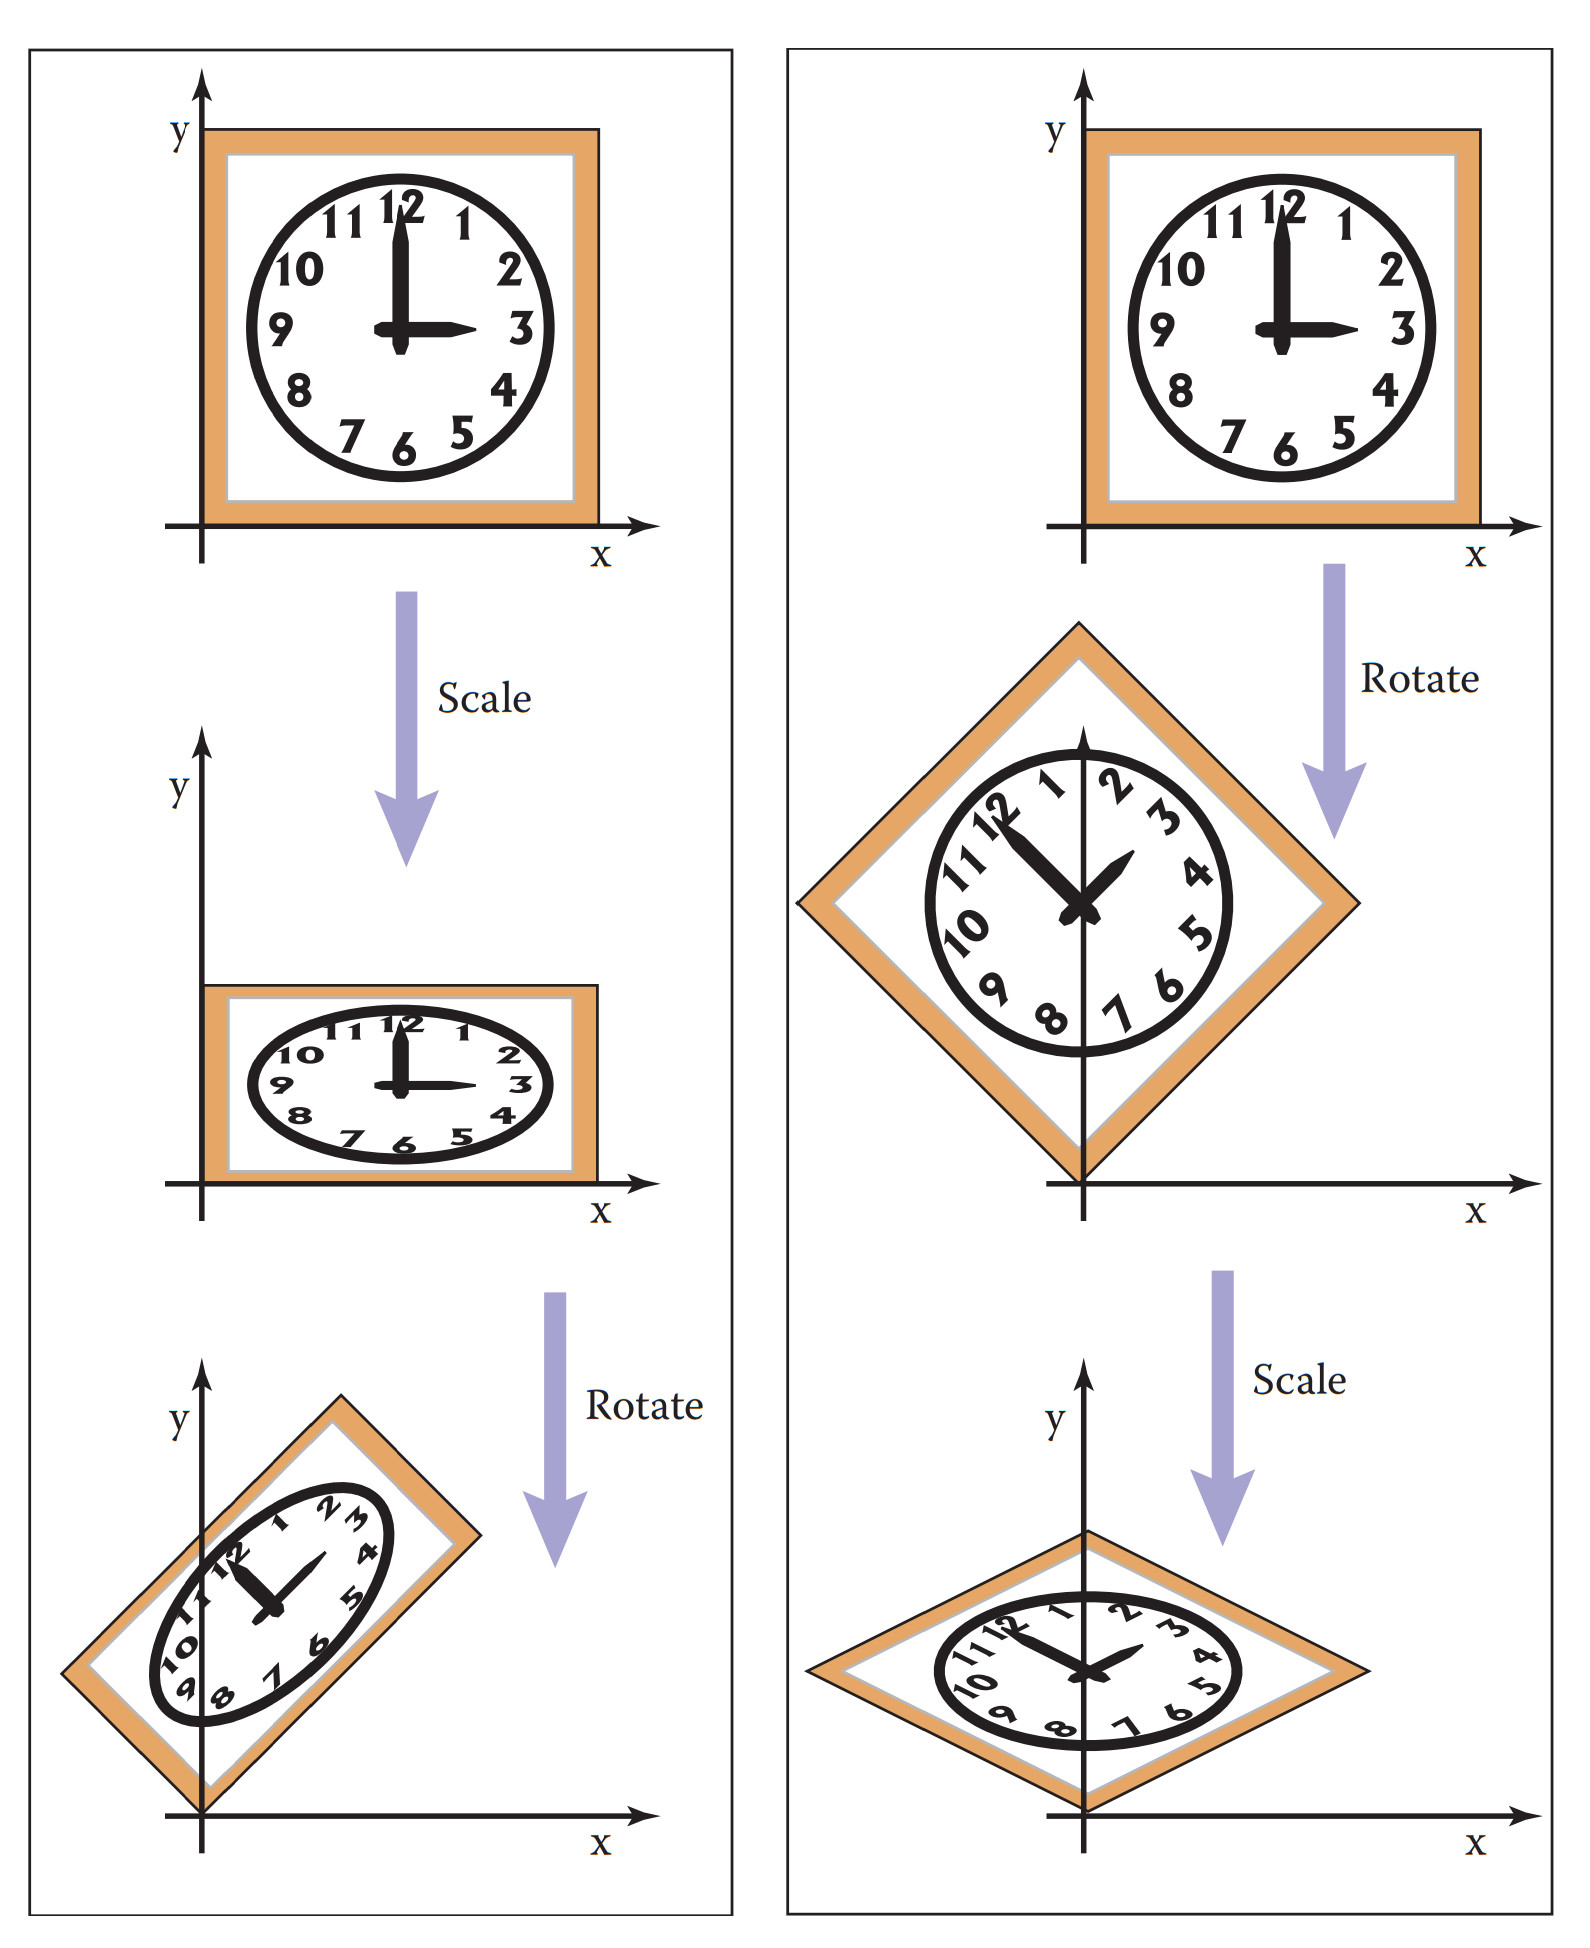
\includegraphics[scale=0.55]{Figure7.11.png}
	\caption{应用两种变换的顺序通常很重要。对于这个例子,我们在y轴上做了二分之一的缩放,然后旋转了$45^{\circ}$。将这两个变换的顺序颠倒一下,会产生不同的结果。}
	\label{fig:7.11}
\end{figure}	

\end{example}

\begin{example}
	使用我们提出的缩放矩阵,非均匀缩放只能沿坐标轴进行。如果我们想拉伸沿着时钟的一条对角线拉伸时钟50\%,使8:00到1:00移动到西北方向,2:00到7:00移动到东南方向,我们可以使用一个结合了轴对齐缩放矩阵的旋转矩阵来达到这个目的。其想法是使用旋转将缩放轴与坐标轴对齐,然后沿该轴缩放,然后旋转回来。在我们的示例中,缩放轴是正方形的“反斜杠”对角线,我们可以使其与$x$轴平行,旋转$+45^{\circ}$。将这些操作放在一起,完整的变换矩阵是:
	
	\begin{equation}
		\operatorname{rotate}\left(-45^{\circ}\right) \operatorname{scale}(1.5,1) \operatorname{rotate}\left(45^{\circ}\right)
		\nonumber
	\end{equation}
	
	在数学符号中,这可以写成$\mathbf{R}\mathbf{S}\mathbf{R}^{\mathbf{T}}$。将三个矩阵相乘的结果是:
	
	\begin{equation}
		\left[\begin{array}{cc}
			1.25 & -0.25 \\
			-0.25 & 1.25
		\end{array}\right]
	\nonumber
	\end{equation}
	
	从旋转和缩放变换中建立起的变换实际上对任何线性变换都是有效的,这诱导我们对这些变换进行强烈的思考,在下一节将进行探讨。
	
\end{example}

\subsection{变换的分解(Decomposition of Transformations)}

有时有必要 "撤销 "一个变换的组合,把一个变换拆成更简单的部分。例如,相对于单独的旋转和缩放,以变换矩阵的形式呈现给用户进行操作通常是有用的,但是一个变换可能被简单地表示为一个矩阵,旋转和缩放已经混合在一起。如果可以通过计算将矩阵分解成所需的部分,调整这些部分,并通过将这些部分再次相乘来重新组装矩阵,就可以实现这种操作。

事实证明,这种分解或矩阵分解是可能的,不管矩阵中的内容是什么。这提供了一种很有效的方式来思考变换以及它们对变换的几何体所做的操作。

\subsubsection*{\textcolor{structure3}{对称特征值分解(Symmetric Eigenvalue Decomposition)}}

让我们从对称阵开始。还记得第\ref{6.4}小节说过,对称阵总是可以通过特征值分解以下矩阵相乘的形式:

\begin{equation}
    \mathbf{A} = \mathbf{R}\mathbf{S}\mathbf{R}^{\mathbf{T}}
    \nonumber
\end{equation}

其中,$\mathbf{R}$是正交阵,$\mathbf{S}$是对角阵;我们称$\mathbf{R}$的列(特征向量)为$\mathbf{v}_{1}$和$\mathbf{v}_{2}$,称$\mathbf{S}$的对象项为$\lambda_{1}$和$\lambda_{2}$。

在几何术语中,我们现在可以认出$\mathbf{R}$是旋转变换,$\mathbf{S}$是缩放变换,因此这只是一个多步骤的几何变换(图\ref{fig:7.12}):

\begin{figure}[htbp]
	\centering
	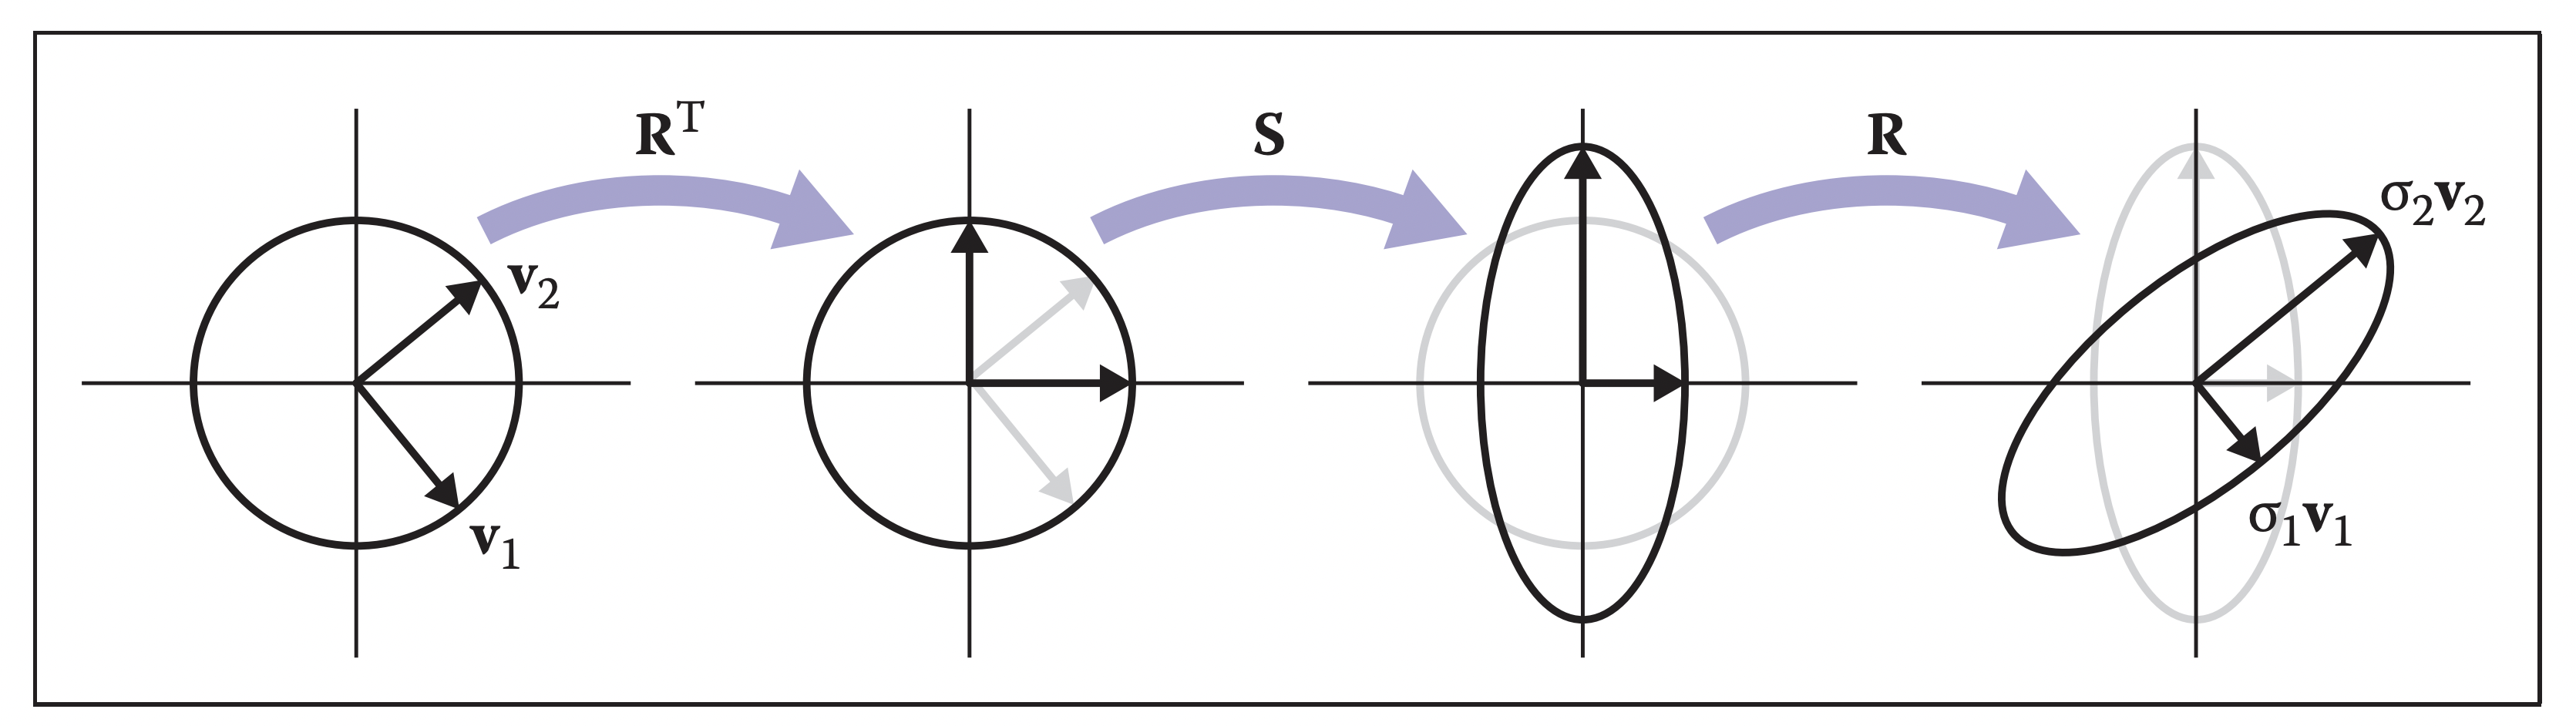
\includegraphics[scale=0.25]{Figure7.12.png}
	\caption{。}
	\label{fig:7.12}
\end{figure}	

\begin{enumerate}
	\item 将$\mathbf{v}_{1}$和$\mathbf{v}_{2}$旋转到$x$轴和$y$轴上(通过旋转矩阵$\mathbf{R}^{T}$)
	
\end{enumerate}










\chapter{视图}
\label{chap08}



\chapter{图形管线}
\label{chap09}

\chapter{信号处理}
\label{chap10}

\chapter{纹理映射}
\label{chap11}

\chapter{图形学的数据结构}
\label{chap12}

\chapter{采样}
\label{chap13}

\chapter{基于物理的渲染}
\label{chap14}

\chapter{ 曲线 }
\label{chap15}



\chapter{电脑动画}
\label{chap16}

\chapter{使用图形硬件}
\label{chap17}

















\chapter{色彩}
\label{chap18}



\chapter{视觉感知}
\label{chap19}

\chapter{色调重现}
\label{chap20}


\chapter{隐式建模}
\label{chap21}

\chapter{游戏中的计算机图形学}
\label{chap22}

\chapter{可视化}
\label{chap23}





\end{document}